\documentclass[hyperref, beleg, german]{cgvpub}
% other document types next to bachelorofscience:
% masterofscience
% diplominf
% diplomist
% beleg

%more options (to be appended in the square brackets):
% german....... german version 
% female........ to be used for female endings in german
% bibnum....... numerical reference style
% final............ intended for the final submission
% lof.............. genereate list of figures
% lot.............. generate list of tables
% noproblem.. do not show task
% notoc......... do not generate table of contents
% twoside...... two sided layout

%\usepackage[ngerman]{babel}
\usepackage{fontawesome5}
\usepackage{enumitem}
\usepackage{verbatim}
\usepackage{siunitx}
\usepackage{tikz, tikz-3dplot, tikz-uml}
\usepackage{pgffor}

\usetikzlibrary{calc, intersections, shapes, positioning}

\sisetup{locale = DE}

\author{Mario Henze}
\title{Layered Depth Images als Ad hoc Rendering für Punktwolken}
\birthday{19. July 1994}
\placeofbirth{Wernigerode}
\matno{4039602}
\betreuer{Dr.\ B.\ Russig}
\bibfiles{literature}
\problem{
VR environments become more and more important in visualization and engineering
applications. In order to provide a comfortable experience without risk of
motion sickness a rendering framerate of 90fps needs to be ensured. Framerate is
even more important than image quality. The goal of this thesis is the
development of an incremental rendering approach for large point cloud data that
can guarantee the necessary framerate by rendering only a subset of the points
per frame and by accumulation information over several frames.

The specific tasks are:
\begin{itemize}
\item Literature research on point cloud rendering and incremental rendering
	approaches
\item Justified selection of an incremental rendering approach for basic point
	cloud rendering that guarantees a user-defined framerate and converges
	to a good approximation of a non-incremental rendering without framerate
	limitations.
\item Implementation of the selected approach in a plugin to the CGV framework
\item Evaluation of the achieved image quality for stereoscopic rendering at
	90fps with a suitable image quality metric for several point clouds of
	different sizes in comparison to a non-incremental rendering approach.
\end{itemize}

Optional Tasks:
\begin{itemize}
\item Optimization of the rendering approach for stereoscopic render
\item Implementation of an advanced hole-free point cloud rendering approach
\end{itemize}
}
\copyrighterklaerung{
	Die Verwendung des CGV Frameworks erfolgt nach den folgenden Lizenzbedingungen:

	Copyright (c) 2016, Stefan Gumhold
	All rights reserved.

Redistribution and use in source and binary forms, with or without
modification, are permitted provided that the following conditions are met:

\begin{itemize}
    \item Redistributions of source code must retain the above
    copyright notice, this list of conditions and the following disclaimer.
    \item Redistributions in binary form must reproduce the above copyright
    notice, this list of conditions and the following disclaimer in the
    documentation and/or other materials provided with the distribution.
    \item Neither the name of the Technische Universitaet Dresden nor the names
    of its contributors may be used to endorse or promote products derived from
    this software without specific prior written permission.
\end{itemize}

THIS SOFTWARE IS PROVIDED BY THE COPYRIGHT HOLDERS AND CONTRIBUTORS ``AS IS''
AND ANY EXPRESS OR IMPLIED WARRANTIES, INCLUDING, BUT NOT LIMITED TO, THE
IMPLIED WARRANTIES OF MERCHANTABILITY AND FITNESS FOR A PARTICULAR PURPOSE ARE
DISCLAIMED.\@ IN NO EVENT SHALL THE COPYRIGHT HOLDER OR CONTRIBUTORS BE LIABLE
FOR ANY DIRECT, INDIRECT, INCIDENTAL, SPECIAL, EXEMPLARY, OR CONSEQUENTIAL
DAMAGES (INCLUDING, BUT NOT LIMITED TO, PROCUREMENT OF SUBSTITUTE GOODS OR
SERVICES;\@ LOSS OF USE, DATA, OR PROFITS;\@ OR BUSINESS INTERRUPTION) HOWEVER
CAUSED AND ON ANY THEORY OF LIABILITY, WHETHER IN CONTRACT, STRICT LIABILITY,
OR TORT (INCLUDING NEGLIGENCE OR OTHERWISE) ARISING IN ANY WAY OUT OF THE USE
OF THIS SOFTWARE, EVEN IF ADVISED OF THE POSSIBILITY OF SUCH DAMAGE.\@
}

\acknowledgments{Ich möchte hiermit meinem Betreuer Dr.\ Benjamin Russig für
die vielen konstruktiven Hinweise danken. Besonders die zielgerichtete Hilfe im
Umgang mit dem CGV Framework waren von immensem Wert.}

\abstracten{abstract text english}
\abstractde{ abstract text german}
\begin{document}

\chapter{Einleitung}%
\label{sec:einleitung}

Der Prozess der Punktwolkenakquisition ist durch technologische Fortschritte
mittlerweile für eine große Anzahl an Problemstellungen machbar und
kostengünstig. So sind bereits Geräte wie die Xbox Kinect oder Intel
Realsense, die selbst für Privatpersonen erschwinglich sind, in der Lage,
Tiefeninformationen zu erfassen und letztendlich Punktwolken zu generieren. Mit
dem Aufkommen von Head Mounted Displays wie der Oculus Rift oder HTC Vive
existieren nun auch Darstellungsmöglichkeiten, die die gewonnen
Tiefeninformationen der menschlichen Wahrnehmung direkter und intuitiver
zugänglich machen.

Die Bildsynthese und Wiedergabe in solchen HMD Systemen stellt jedoch besondere
Vorgaben in Hinblick auf Benutzbarkeit. So muss jederzeit sichergestellt
werden, dass die Immersion dieser Virtual Reality Umgebung erhalten bleibt. Das
bedeutet es herrschen harte Schranken für Eingabeverzögerung und
Bildwiederholfrequenz und deren Übertretung hat den Verlust von Interaktivität
und im schlimmsten Fall physiologische Probleme wie Motion Sickness zur Folge.

In dieser Arbeit soll ein Verfahren zur interaktiven Darstellung von
Punktwolken entwickelt werden, welches in Hinblick auf die genannten Probleme
optimiert ist. So besteht das Ziel darin, selbst größte Datensätze noch in
interaktiver Weise darzustellen. Dazu werden zunächst Ansätze zur klassischen
Punktwolken Darstellung und zum inkrementellen Rendering vorgestellt und deren
Kombinationsmöglichkeiten untersucht. In einem weiteren Schritt soll, das so
entwickelte Verfahren als C++ Plugin für das cgv-Framework des Lehrstuhls
umgesetzt werden. Abschließend werden die gewonnen Erfahrungen in Bezug auf
Laufzeitverhalten und Implementation dargelegt und erklärt.

\chapter{Verwandte Arbeiten}%
\label{sec:verwandte_arbeiten}

\section{Überblick}

Das Ziel dieser Arbeit besteht darin, einen hybriden Renderingprozess zu
entwerfen, welcher temporale Redundanz als zusätzliche Optimierung in einen
klassischen Punktwolkenrenderer einfügt. Um dies zu erreichen, werden in den
folgenden Abschnitten zunächst sog.\ Image-based Rendering Verfahren
vorgestellt. Diese Algorithmen werden hauptsächlich zur Interpolation von neuen
Bildern aus bereits Bekannten benutzt. Danach werden klassische
Renderingverfahren für Punktwolken vorgestellt.

\section{Image-based Rendering}

Im Bereich des Image-based Rendering kann die Arbeit~\cite{shum2000review} als
Überblick gesehen werden. Heung-Yeung und Sing Bing arbeiten hierbei die
unterschiedliche Verwendung von geometrischen Informationen bei verschiedenen
Bildsyntheseverfahren heraus. So wird zunächst eine plenoptische Funktion
definiert, welche als Grundlage der geometrielosen Verfahren genutzt wird. In
der Mitte des Spektrums sind Methoden mit impliziter Geometrieinformation
aufgeführt. In diese Kategorie fallen View-Morphing und Transfermethoden,
welche die geometrische Redundanz zweier aufeinanderfolgender Bilder ausnutzen.
Zuletzt werden auch die klassischen Verfahren der Bildsynthese, welche auf
explizite Geometrie wie Dreiecksnetze aufsetzen, eingeordnet.

In~\cite{chang1999ldi} stellen Chun-Fa et al.\ basierend auf~\cite{he1998layered}
eine Datenstruktur vor, welche zur Organisation von Referenzbildern mit
variierender Tiefenauflösung genutzt werden können. So werden Bilder aus
verschieden Perspektiven in einen sog. Layered Depth Tree eingfügt. Da bei
gleicher Auflösung Referenzbilder aus einer näheren Perspektive
Tiefeninformationen höher abtasten als Entferntere, können diese in einen Octree
eingeordnet werden und es entsteht eine Art Ordnungsrelation. Mithilfe dieser
Datenstruktur ist es nun möglich, die Referenzbilder auswählen, deren
Tiefenauflösung in etwa dem zu synthetisierenden Bildausschnitts entspricht. In
der praktischen Umsetzung zeigen Chun-Fa et al.\ auf, dass der Speicherverbrauch
nicht wesentlich höher als die direkte Speicherung aller Referenzbilder ist und
auch die Rechenzeit im schlimmsten Fall gleich dem direkten Rendern aller
Referenzbilder ist.

Ein generelles Vorgehen beim Warpen von 3D Renderings wird von Mark et al.\
in~\cite{mark1997post} vorgestellt. So wird die These untersucht, dass ein Paar
von gerenderten Bildern und deren entsprechende Tiefenpuffer ausreichen um
beliebige Ansichten aus benachbarten Perspektiven zu zeichnen. Unter
Zuhilfenahme der in~\cite{mcmillan1995head} formulierten Morphing Gleichung
wird eine Korrespondenz zwischen beiden Bildern hergestellt und ein
kombiniertes Bild an einer neuen Position erzeugt. Anschließend werden
verschiedene Probleme des Verfahrens aufgezeigt. So entstehen beim
bildbasierten Morphing partielle und totale Verdeckungsartefakte. Die in Bezug
zum Betrachter variierende diskrete Abtastung von Oberflächen führt weiterhin
zur Entstehung von Löchern. Um diese Effekte auszugleichen werden mehrere
Strategien vorgestellt, welche auf der Rekonstruktion von Geometrie und
optimierter Interpolation basieren.

\section{Klassische Punktwolkenrenderer}

Mit QSplat wurde ein einflussreiches Verfahren zum Zeichnen von Punktwolken von
Rusinkiewicz und Levoy in~\cite{rusinkiewicz2000qsplat} entwickelt. Hierbei
wird das effiziente Rendern durch die Verwendung einer Hierarchie von
Begrenzungskugeln ermöglicht. In einem Vorverarbeitungsschritt wird zunächst
ein Dreiecksnetz genutzt um bei der Bestimmung der Begrenzungskugeln
Oberflächennormalen einzubeziehen und Lochartefakte unterbinden zu können.
Anschließend kann die Hierarchie durch eine rekursive Durchquerung gezeichnet
werden. Dabei werden alle Pfade bei Verfehlen eines Sichtbarkeitskriteriums
verworfen. Des Weiteren werden der Einfluss von verschiedenen Splatting Formen
auf die Bildqualität untersucht und die Laufzeit von Vorverarbeitung und
Rendering aufgeschlüsselt.

Goswami et al.\ benutzen einen variablen Detailgrad beim Zeichnen und eine
Baumstruktur zur Verwaltung der Punktwolke~\cite{goswami2010high}. Grundlegend
muss bei diesem Verfahren zunächst eine Vereinfachung und Zusammenfassung der
Punkte erfolgen. Dafür werden verschieden große Cluster in Abhängigkeit der
lokalen Varianz erzeugt und in einen KD Baum eingefügt. Eine Quantisierung des
Datenraums entlang der Koordinatenachsen ermöglicht weiterhin eine schnelle
Umsetzung dieses Prozesses, da jede Zelle parallel bearbeitet werden kann. Für
das Rendering werden alle Knoten dieses LOD-Baums in eine
Prioritätswarteschlange nach ihrem Detailgrad eingeordnet. Beginnend vom
Wurzelknoten werden solange Cluster expandiert bis eine ausreichende
Punktdichte erreicht ist.

Eine weitere Implementation mit Fokus auf Virtual Reality wird von Discher et
al.\ in~\cite{discher2018point} vorgestellt. Das Punktwolkenrendering wird
dabei in drei Phasen eingeteilt. Zunächst wird eine sog.\ repräsentative
Untermenge in Abhängigkeit der Auslastung von CPU und GPU ausgewählt. Nach dem
Entfernen von Punkten außerhalb des Sichtkegelstumpfes und überflüssigen
Details wird ein KD Baum aufgebaut. Das Renderen erfolgt dann in G-Buffer
(siehe~\cite{saito1990comprehensible}), welche bestimmte geometrische
Eigenschaften wie Tiefe oder Oberflächennormalen als Zwischenbild abspeichern.
Die Anwendung dieser Zwischentexturen ermöglicht abschließend eine
Bildnachbearbeitung. Dieser finale Schritt dient dazu die Bildqualität
nachträglich zu steigern. Zum Beispiel können Löcher gefüllt, Aliasing
Artefakte beseitigt und Kanten besonders hervorgehoben werden. Außerdem wurden
mehrere Kompositionsansätze für die anschließende Bildsynthese untersucht und
deren Laufzeitperformance evaluiert.

Wimmer und Scheiblauer entwickeln in~\cite{wimmer2006instant} ein Verfahren,
dass ohne Vorverarbeitung eine möglichst große Menge an Punkten mit
interaktiven Bildraten darstellen soll. Zur Umsetzung werden Memory Optimized
Sequential Point Trees (MOSPT) und verschachtelte Octrees als Datenstrukturen
vorgestellt. Dies ermöglicht ein serielles Rendern der Punktwolke nach dem out
of core Prinzip. Um eine lokale Zusammenfassung von Punkten und damit eine
Datenreduktion zu erreichen wird eine Fehlermetrik eingeführt, die zur
Sortierung der MOSPT genutzt wird. Die so gewonnene Hierarchie ermöglicht nun
das Verwerfen von Knoten mit zu geringem Einfluss auf das resultierende Bild.
Für den Rendervorgang wird zunächst ein Intervall auf der Fehlermetrik bestimmt
und dann alle entsprechenden Knoten des MOSPT gezeichnet. Da die Nutzung eines
einzelnen MOSPT statische Vorraussetzungen wie ein globales LOD fordern, wird
nur ein Teil der Punktwolken in diesen angeordnet. Diese Teilmengen werden
wiederum in einen Octree eingefügt. Abschließend wird der Laufzeitvorteil der
MOSPT untersucht und auf Artefakte des Renderingprozesses eingegangen.

\section{Einordnung des Renderingansatzes}

Wie in Abschnitt~\ref{sec:verwandte_arbeiten} aufgezeigt, existieren eine
Vielzahl an Renderverfahren für Punktwolken und bildbasierten Morphing
Ansätzen. Das Ziel dieser Arbeit besteht darin eine Kombination dieser beiden
Vorgehen zu entwickeln, welche sowohl ein schnelles Zeichnen von
unverarbeiteten Punktwolken als auch eine Wiederverwendung von bereits
gezeichneten Bildbereichen ermöglicht.

Zunächst ist hervorzuheben, dass der Großteil der Punktzeichnungs Algorithmen
eine Vorverarbeitung der Punktwolke vorrausetzt. So ist zu erkennen, dass
generell Artefakte der Punktwolkenakquisition ausgeglichen und eine
Speicherzugriff optimierende Datenstruktur erreicht werden soll. Hierfür wird
fast ausschließlich die räumlich variierende Punktdichte zum Clustering
genutzt. Anschließend wird eine Baumstruktur aufgebaut, welche das rekursive
Zeichnen bis zu einem ausreichenden Detailgrad ermöglicht. Da die vorliegende
Arbeit jedoch darauf abzielt, zu einem späteren Zeitpunkt kontinuierlich
erfasste Punkte in die Darstellung einfließen zu lassen, ist ein aufwendiges
Verarbeiten nicht möglich. So liegt der Zeitaufwand von
QSplat~\cite{rusinkiewicz2000qsplat} beim Preprocessing einer Wolke mit rund
127 Millionen Punkten bei einer knappen Stunde. Selbst modernere Ansätze
wie~\cite{goswami2010high} benötigen für diesen Verarbeitungsschritt immer noch
mehrere Minuten. Auch wenn diese Angaben aufgrund von unterschiedlicher
Hardware nicht direkt vergleichbar sind, geben sie eine Größenordnung der zu
erwartenden Laufzeitkosten an.

Betrachtet man die Problemstellungen jedoch aus Sicht des bildbasierten
Morphings, verspricht die Umsetzung des Renderingprozesses als Layered Depth
Image analog zu~\cite{chang1999ldi} einen Vorteil. So werden in dem LDI
Bildpunkte mit verschiedenen Tiefen gespeichert. Außerdem ist eine elegante
Interpolation zwischen verschiedenen Referenzen durch die Morphing Gleichung
von McMillan (siehe~\cite{mcmillan1995list} und~\cite{mcmillan1995plenoptic})
möglich. Unter der Annahmen, dass die globalen Punkte der Wolke äquivalent zu
den relativen Punkten des LDIs sind, kann das Rendern von Punktwolken in ein
Rendern von LDIs überführt werden. Das bedeutet, der einzige
Vorverarbeitungsschritt der Punktdaten besteht darin, die Punkte aus dem
globalen Koordinatensystem in das kamerabezogene System zu transformieren.

Außerdem ist festzustellen, dass bei der Anwendung von HMDs eine ständige
Veränderung der Kameraposition durch die teilweise willkürlichen Bewegungen des
menschlichen Kopfes auftreten. Somit sind Renderverfahren von Vorteil, die eine
schnelle Interpolation von benachbarten Ansichten ermöglichen. Da auch dieses
Kriterium durch die LDIs abgedeckt wird, baut die folgende Implementation auf
Basis dieser Festlegungen einen eigenen Rendervorgang auf.

\chapter{Theoretische Betrachtungen}

\section{Lochkamera}

\begin{figure}
	\centering
	\tdplotsetmaincoords{70}{110}
	\begin{tikzpicture}[
        tdplot_main_coords,
        poi/.style = {circle, inner sep=1.5pt}
    ]
    %\draw[->] (0, 0, 0) -- (8, 0, 0) node[anchor = north]{x};
    %\draw[->] (0, 0, 0) -- (0, 8, 0) node[anchor = west]{y};
    %\draw[->] (0, 0, 0) -- (0, 0, 8) node[anchor = south]{z};
    \node[poi, fill=gray, label=below:{Brennpunkt}] (focal) at (0, 0, 0) {};
    % image corners
    \node[poi, fill=red] (ul) at (-4, 10, 2.25) {};
    \node[poi, fill=blue] (ur) at (4, 10, 2.25) {};
    \node[poi, fill=green] (lr) at (4, 10, -2.25) {};
    \node[poi, fill=yellow] (ll) at (-4, 10, -2.25) {};
    % sensor corners
    \node[poi, fill=red] (sul) at (-2, 5, 1.125) {};
    \node[poi, fill=blue] (sur) at (2, 5, 1.125) {};
    \node[poi, fill=green] (slr) at (2, 5, -1.125) {};
    \node[poi, fill=yellow] (sll) at (-2, 5, -1.125) {};
    % projection corners
    \node[poi, fill=green] (pul) at (-2, -5, 1.125) {};
    \node[poi, fill=yellow] (pur) at (2, -5, 1.125) {};
    \node[poi, fill=red] (plr) at (2, -5, -1.125) {};
    \node[poi, fill=blue] (pll) at (-2, -5, -1.125) {};
    % coords of image
    %\draw[->] (focal) -- (ul);
    %\draw[->] (ul) -- ++(2,0,0);
    %\draw[->] (ul) -- ++(0,0,-2);
    % image borders
    \draw (ul) -- (ur);
    \draw (ll) -- (lr);
    \draw (ul) -- (ll);
    \draw (ur) -- (lr);
    % view frustum
    \draw (focal) -- (sul);
    \draw (focal) -- (sur);
    \draw (focal) -- (slr);
    \draw (focal) -- (sll);
    \draw (sul) -- (ul);
    \draw (sur) -- (ur);
    \draw (slr) -- (lr);
    \draw (sll) -- (ll);
    % sensor edges
    \draw (sul) -- (sur);
    \draw (sll) -- (slr);
    \draw (sul) -- (sll);
    \draw (sur) -- (slr);
    % projection edges
    \draw[dotted] (pul) -- (pur);
    \draw[dotted] (pll) -- (plr);
    \draw[dotted] (pul) -- (pll);
    \draw[dotted] (pur) -- (plr);
    % view frustum
    \draw[dotted] (focal) -- (pul);
    \draw[dotted] (focal) -- (pur);
    \draw[dotted] (focal) -- (plr);
    \draw[dotted] (focal) -- (pll);
\end{tikzpicture}
	\caption{Abbildungsverhältnisse einer Lochkamera auf Sensor- und reale
		Bildebene}%
	\label{fig:pinholecamera}
\end{figure}

Da LDIs prinzipbedingt auf den Betrachter bezogen definiert sind und einer
Perspektivtransformation unterliegen, ist die Definition einer Lochkamera
sinnvoll. So kann die Lochkamera als idealisierte optische Kamera aufgefasst
werden, welche alle Sichtstrahlen in aus der Szene in einem einzigen Punkt
bündelt (siehe Abbildung~\ref{fig:pinholecamera}). Bei praktischen Aufbauten
einer Lochkamera wird das projizierte Bild hinter diesem Brennpunkt gespiegelt
auf einer Ebene abgebildet. Zur Vereinfachung wird auf diesen Umstand
verzichtet und die Bildebene kurz vor dem Brennpunkt zwischen Szene und
Koordinatenursprung der Kamera platziert. Dadurch wird auch die Spieglung der
Abbildung verhindert und die geometrischen Zusammenhänge können mit einfachen
Strahlensätzen interpretiert werden. In Anlehnung an digitale Linsenkameras
wird diese Ebene im Quellcode auch als Sensorebene bezeichnet. Des Weiteren
definiert die Lochkamera mit ihrem Öffnungswinkel und ihrem Seitenverhältnis
einen Sichtkegelstumpf.

\section{Plenoptic Modelling}

Um neuartige Renderansätze zu entwickeln, ist es notwendig eine präzise
Definition der Szene zu finden. Dafür bietet sich die plenoptische Modellierung
an. Hierbei wird zunächst versucht, die Szene unabhängig vom Beobachter zu
beschreiben. Adelson und Bergen definieren dafür in~\cite{adelson1991plenoptic}
die plenoptische Funktion wie folgt:

\begin{equation}
	P_7 = P(V_x, V_y, V_z, \theta, \Phi, \lambda, t)
\end{equation}

\begin{description}[style=sameline]
	\item[\( V_x, V_y, V_z \)] mögliche Position der Kamera
	\item[\( \theta, \Phi \)] Winkel eines Sichtstrahls
	\item[\( \lambda \)] Wellenlänge des Lichts
	\item[\( t \)] Zeitpunkt der Beobachtung
\end{description}

Diese Form der Beschreibung ermöglicht es, die Szene zu jedem Zeitpunkt an
jeder Stelle und aus jeder Richtung zu samplen. Anhand dieses generellen
Modells können nun Vereinfachungen vorgenommen werden.

Es ist zunächst festzustellen, dass Punktwolkendaten in einem globalen
Koordinatensystem gegeben sind. Beim Punktwolkenrendering gehen jedoch nur die
sichtbaren Punkte in das Bild ein. Außerdem erfolgt die Kamerabewegung von HMDs
ausschließlich kontinuierlich. Daraus folgt, dass die Untermengen aller
sichtbaren Punkte zwischen zwei gerenderten Ansichten nahezu identisch sind.
Ähnliche Annahmen liegen auch dem Modell der Layered Depth Images zugrunde.

McMillan und Bishop ermöglichen in~\cite{mcmillan1995plenoptic} unter
Ausschluss von \( t \) und \( \lambda \) das plenoptische Modellieren. So
ergibt sich durch die Annahme einer statischen Szene:

\begin{equation}
	P_5 = P(V_x, V_y, V_z, \theta, \Phi)
\end{equation}

In diesem Kontext kann ein gewöhnliches Bild als unvollständige Abtastung der
plenoptischen Funktion an einem festen Betrachtungspunkt aufgefasst werden. Die
zentrale Fragestellung des Image-based Renderings besteht also darin, aus einer
Menge von unvollständigen und diskreten Abtastungen die kontinuierliche
plenoptische Funktion zu rekonstruieren~\cite{mcmillan1995plenoptic}.

\section{Layered Depth Image}

\begin{figure}
	\centering
	\tdplotsetmaincoords{70}{110}
	\begin{tikzpicture}[
        tdplot_main_coords,
        poi/.style = {draw, shape = circle}
    ]
    %\draw[->] (0, 0, 0) -- (8, 0, 0) node[anchor = north]{x};
    %\draw[->] (0, 0, 0) -- (0, 8, 0) node[anchor = west]{y};
    %\draw[->] (0, 0, 0) -- (0, 0, 8) node[anchor = south]{z};
    \node (focal) at (0, 0, 0) {};
    % image corners
    \node (ul) at (-4, 10, 2.25) {};
    \node (ur) at (4, 10, 2.25) {};
    \node (lr) at (4, 10, -2.25) {};
    \node (ll) at (-4, 10, -2.25) {};
    % sensor corners
    \node (sul) at (-2, 5, 1.125) {};
    \node (sur) at (2, 5, 1.125) {};
    \node (slr) at (2, 5, -1.125) {};
    \node (sll) at (-2, 5, -1.125) {};
    % coords of image
    %\draw[->] (focal) -- (ul);
    %\draw[->] (ul) -- ++(2,0,0);
    %\draw[->] (ul) -- ++(0,0,-2);
    % image borders
    \draw[dotted] (ul.center) -- (ur.center);
    \draw[dotted] (ll.center) -- (lr.center);
    \draw[dotted] (ul.center) -- (ll.center);
    \draw[dotted] (ur.center) -- (lr.center);
    % view frustum
    \draw[dotted] (focal.center) -- (sul.center);
    \draw[dotted] (focal.center) -- (sur.center);
    \draw[dotted] (focal.center) -- (slr.center);
    \draw[dotted] (focal.center) -- (sll.center);
    \draw[dotted] (sul.center) -- (ul.center);
    \draw[dotted] (sur.center) -- (ur.center);
    \draw[dotted] (slr.center) -- (lr.center);
    \draw[dotted] (sll.center) -- (ll.center);
    % sensor edges
    \draw[] (sul.center) -- (sur.center);
    \draw[] (sll.center) -- (slr.center);
    \draw[] (sul.center) -- (sll.center);
    \draw[] (sur.center) -- (slr.center);
    % sensor grid
    %\draw[dotted] ($ (sul)!.25!(sll) $) -- ($ (sur)!.25!(slr) $);
    \foreach \n in {1,...,8}{
        \draw[] ($ (sul)!.125*\n!(sll) $) -- ($ (sur)!.125*\n!(slr) $);};
    \foreach \n in {1,...,16}{
        \draw[] ($ (sul)!.0625*\n!(sur) $) -- ($ (sll)!.0625*\n!(slr) $);};
    % world grid
    %\draw[dotted] ($ (sul)!.25!(sll) $) -- ($ (sur)!.25!(slr) $);
    \foreach \n in {1,...,8}{
        \draw[dotted] ($ (ul)!.125*\n!(ll) $) -- ($ (ur)!.125*\n!(lr) $);};
    \foreach \n in {1,...,16}{
        \draw[dotted] ($ (ul)!.0625*\n!(ur) $) -- ($ (ll)!.0625*\n!(lr) $);};
    % first example ray --> "f" as prefix
    % highlight sensor cell
    % calculate points on border
    \node (fslb1) at ($ (sul)!.125*1!(sll) $) {};
    \node (fslb2) at ($ (sul)!.125*2!(sll) $) {};
    \node (fsrb1) at ($ (sur)!.125*1!(slr) $) {};
    \node (fsrb2) at ($ (sur)!.125*2!(slr) $) {};

    \node (fsul) at ($ (fslb1)!.0625*1!(fsrb1) $) {};
    \node (fsll) at ($ (fslb2)!.0625*1!(fsrb2) $) {};
    \node (fslr) at ($ (fslb2)!.0625*2!(fsrb2) $) {};
    \node (fsur) at ($ (fslb1)!.0625*2!(fsrb1) $) {};
    \filldraw[draw=red, fill=red!20] (fsul.center) -- (fsll.center) -- (fslr.center) -- (fsur.center) -- cycle;
    % highlight world cell
    % calculate points on border
    \node (flb1) at ($ (ul)!.125*1!(ll) $) {};
    \node (flb2) at ($ (ul)!.125*2!(ll) $) {};
    \node (frb1) at ($ (ur)!.125*1!(lr) $) {};
    \node (frb2) at ($ (ur)!.125*2!(lr) $) {};

    \node (ful) at ($ (flb1)!.0625*1!(frb1) $) {};
    \node (fll) at ($ (flb2)!.0625*1!(frb2) $) {};
    \node (flr) at ($ (flb2)!.0625*2!(frb2) $) {};
    \node (fur) at ($ (flb1)!.0625*2!(frb1) $) {};
    \filldraw[draw=red, fill=red!20] (ful.center) -- (fll.center) -- (flr.center) -- (fur.center) -- cycle;

    % another example ray --> "a" as prefix
    % highlight sensor cell
    % calculate points on border
    \node (aslb1) at ($ (sul)!.125*5!(sll) $) {};
    \node (aslb2) at ($ (sul)!.125*6!(sll) $) {};
    \node (asrb1) at ($ (sur)!.125*5!(slr) $) {};
    \node (asrb2) at ($ (sur)!.125*6!(slr) $) {};

    \node (asul) at ($ (aslb1)!.0625*11!(asrb1) $) {};
    \node (asll) at ($ (aslb2)!.0625*11!(asrb2) $) {};
    \node (aslr) at ($ (aslb2)!.0625*12!(asrb2) $) {};
    \node (asur) at ($ (aslb1)!.0625*12!(asrb1) $) {};
    \filldraw[draw=red, fill=red!20] (asul.center) -- (asll.center) -- (aslr.center) -- (asur.center) -- cycle;
    % highlight world cell
    % calculate points on border
    \node (alb1) at ($ (ul)!.125*5!(ll) $) {};
    \node (alb2) at ($ (ul)!.125*6!(ll) $) {};
    \node (arb1) at ($ (ur)!.125*5!(lr) $) {};
    \node (arb2) at ($ (ur)!.125*6!(lr) $) {};

    \node (aul) at ($ (alb1)!.0625*11!(arb1) $) {};
    \node (all) at ($ (alb2)!.0625*11!(arb2) $) {};
    \node (alr) at ($ (alb2)!.0625*12!(arb2) $) {};
    \node (aur) at ($ (alb1)!.0625*12!(arb1) $) {};
    \filldraw[draw=red, fill=red!20] (aul.center) -- (all.center) -- (alr.center) -- (aur.center) -- cycle;

    % the layered pixels
    \node (fsc) at ($ (fsul)!.5!(fslr) $) {}; % first example sensor center
    \node (fwc) at ($ (ful)!.5!(flr) $) {}; % first example world center
    \node (asc) at ($ (asul)!.5!(aslr) $) {}; % another example sensor center
    \node (awc) at ($ (aul)!.5!(alr) $) {}; % another example world center
    \draw[dashed] (fsc.center) -- ($ (fsc.center)!-.25!(fwc.center) $);
    \draw (fsc.center) -- (fwc.center);
    \draw[dashed] (fwc.center) -- ($ (fsc.center)!1.2!(fwc.center) $);
    \node[fill=orange, draw, circle, inner sep=1.5pt, label=above:\(z_1\)]%
        at ($ (fsc)!.1!(fwc)$) {};
    \node[fill=gray, draw, circle, inner sep=1.5pt, label=below:\(z_2\)]%
        at ($ (fsc)!.14!(fwc)$) {};
    \node[fill=green, draw, circle, inner sep=1.5pt, label=above:\(z_3\)]%
        at ($ (fsc)!.3!(fwc)$) {};
    \node[fill=blue, draw, circle, inner sep=1.5pt, label=above:\(z_4\)]%
        at ($ (fsc)!.4!(fwc)$) {};
    \node[fill=purple, draw, circle, inner sep=1.5pt, label=above:\(z_5\)]%
        at ($ (fsc)!.77!(fwc)$) {};
    \draw[dashed] (asc.center) -- ($ (asc.center)!-.2!(awc.center) $);
    \draw (asc.center) -- (awc.center);
    \draw[dashed] (awc.center) -- ($ (asc.center)!1.35!(awc.center) $);
    \node[fill=gray, draw, circle, inner sep=1.5pt, label=below:\(z_6\)]%
        at ($ (asc)!.15!(awc)$) {};
    \node[fill=red, draw, circle, inner sep=1.5pt, label=above:\(z_7\)]%
        at ($ (asc)!.24!(awc)$) {};
    \node[fill=orange, draw, circle, inner sep=1.5pt, label=below:\(z_8\)]%
        at ($ (asc)!.3!(awc)$) {};
    \node[fill=blue, draw, circle, inner sep=1.5pt, label=above:\(z_9\)]%
        at ($ (asc)!.5!(awc)$) {};
    \node[fill=green, draw, circle, inner sep=1.5pt, label=above:\(z_{10}\)]%
        at ($ (asc)!.7!(awc)$) {};
    \node[fill=lightgray, draw, circle, inner sep=1.5pt, label=below:\(z_{11}\)]%
        at ($ (asc)!.75!(awc)$) {};
    \node[fill=purple, draw, circle, inner sep=1.5pt, label=above:\(z_{12}\)]%
        at ($ (asc)!.9!(awc)$) {};
\end{tikzpicture}
	\caption{Veranschaulichung von Punkten in einem LDI.\@ Alle Punkte mit
		gleicher Pixelzugehörigkeit werden zusammenhängend gespeichert. Jeder
		Punkt im Pixel besitzt eine Tiefe \(z\) und eine Farbe \(c\).}%
	\label{fig:layereddepthimage}
\end{figure}

Das Layered Depth Image wurden von Shade et al.\ in~\cite{he1998layered}
vorgestellt. Es fügt sich in die Taxonomie der Abtastungen der plenoptischen
Funktion zwischen Lichtfeldaufnahmen bzw. Lumigraphs und klassische
Kugelpanoramen ein. LDIs wurden entwickelt um generelle Verdeckungsartefakte zu
beseitigen, bei denen konventionelle Sprite Warping Algorithmen versagten.
Hierfür werden die Pixel eines gewöhnlichen Bildpuffers mit Informationen
überbelegt. Es wird sozusagen die Menge aller Pixel in verschieden Tiefen mit
gleicher Bildposition gespeichert (siehe
Abbildung~\ref{fig:layereddepthimage}). Um dieses LDI zu erzeugen werden
mehrere Referenzbilder mit Tiefeninformation erfasst und diese dann in die
Ansicht des LDIs gewarpt.

\begin{figure}
	\centering
	\tdplotsetmaincoords{70}{60}
	\begin{tikzpicture}[
        tdplot_main_coords
    ]
% general world coordinate system
\draw[->, very thick] (0, 0, 0) -- node[below] {\( \hat{\imath} \)} ++ (3, 0, 0);
\draw[->, very thick] (0, 0, 0) -- node[below] {\( \hat{k} \)} ++ (0, 3, 0);
\draw[->, very thick] (0, 0, 0) -- node[left] {\( \hat{\jmath} \)} ++ (0, 0, -3);

% image coordinate system
\node (ul) at (4, 4, 4) {};
\node (ll) at ($ (ul) + (0,.5,-2) $) {};
\node (lr) at ($ (ul) + (4,.5,-2) $) {};
\node (ur) at ($ (ul) + (4,0,0) $) {};
\draw[->, thick] (0, 0, 0) -- node[above] {\(c\)} ++ (ul.center);
\draw[->, thick] (ul.center) -- node[above] {\( \hat{a} \)} ++ (ur);
\draw[->, thick] (ul.center) -- node[left] {\( \hat{b} \)} ++ (ll);

\foreach \n in {0,...,8}{
    \draw[] ($ (ul)!.125*\n!(ll) $) -- ($ (ur)!.125*\n!(lr) $);};
\foreach \n in {0,...,16}{
    \draw[] ($ (ul)!.0625*\n!(ur) $) -- ($ (ll)!.0625*\n!(lr) $);};
\end{tikzpicture}
	\caption{Zusammenhänge im LDI Koordinatensystem. Die Vektoren \( \hat{\imath}
		\), \( \hat{\jmath} \) und \( \hat{k} \) spannen das Weltkoordinatensystem
		auf. Die Vektoren \( \hat{a} \), \( \hat{b} \) sind die Basis LDI
		Bildraums. (Darstellung adaptiert aus~\cite{mcmillan1997image})}%
	\label{fig:ldicoord}
\end{figure}

Wie in~\cite{chang1999ldi} dargelegt, ist die McMillan 3D Morphing Gleichung
(siehe~\cite{mcmillan1995list}~\cite{mcmillan1995plenoptic}) auf das LDI
anwendbar. Um diese definieren zu können muss jedoch zunächst das Kameramodell
nach~\cite{mcmillan1997image} beschrieben werden (siehe
Abbildung~\ref{fig:ldicoord}). Generell befindet sich das LDI in einem
dreidimensionalen euklidischen Raum mit den Basisvektoren \( (\hat{\imath},
\hat{\jmath}, \hat{k}) \). Außerdem wird ein weiteres zweidimensionales
Koordinatensystem durch die Basis \( (\hat{a}, \hat{b}) \) aufgespannt. Allen
gespeicherten Bildpunkten werden Koordinaten in dieser Bildebene zugewiesen.
Ohne Beschränkung der Allgemeinheit wird der Ursprung in eine Ecke des
abgeschlossenen Bildbereiches durch den Vektor \( c \) festgelegt.

Unter der Annahme, dass alle Sichtstrahlen aus den Koordinatenursprung \(
(0,0,0) \) stammen, kann eine direkte Korrespondenz zwischen dem
Richtungsvektor \( \vec{d} \) und den Bildpunkten des LDI definiert werden:
%
\begin{equation}
	\vec{d} =
	\begin{pmatrix}
		d_{\hat{\imath}} \\
		d_{\hat{\jmath}} \\
		d_{\hat{k}}
	\end{pmatrix} =
	\begin{pmatrix}
		a_{\hat{\imath}} &
		b_{\hat{\imath}} &
		c_{\hat{\imath}}   \\
		a_{\hat{\jmath}} &
		b_{\hat{\jmath}} &
		c_{\hat{\jmath}}   \\
		a_{\hat{k}}      &
		b_{\hat{k}}      &
		c_{\hat{k}}        \\
	\end{pmatrix}
	\begin{pmatrix}
		u \\
		v \\
		1
	\end{pmatrix} =
	\mathbf{P}
	\begin{pmatrix}
		u \\
		v \\
		1
	\end{pmatrix}
\end{equation}
%
Hierbei ist jedoch zu beachten, dass alle skalaren Vielfachen der Abbildung \(
\mathbf{P} \) auch eine gültige Transformation ergeben.

\section{Morphing Gleichung}

\begin{figure}
	\centering
	\begin{tikzpicture}
    % positions
    \node[draw, circle, inner sep=1.5pt, label=below:\(C_2\)] (C2) at (0, 0) {};
    \node[draw, circle, inner sep=1.5pt, label=below:\(C_1\)] (C1) at (5, 0) {};
    \node[draw, circle, inner sep=1.5pt, label=above:\(X\)] (X) at (7, 7) {};
    \draw[lightgray, name path=c1x] (C1) -- (X);
    \draw[lightgray, name path=c2x] (C2) -- (X);
    \draw[lightgray] (C2) -- (C1);
    \draw[|<->|] ($(C1)!5mm!-90:(X)$)--node[fill=white] {\(r\)} ($(X)!5mm!90:(C1)$);
    % frustum corners
    \begin{scope}[rotate around={-30:(C2)}]
        \node (c2l) at (-1, 2) {};
        \node (c2r) at (1, 2) {};
    \end{scope}
    \begin{scope}[rotate around={-22:(C1)}]
        \node (c1l) at (4, 2) {};
        \node (c1r) at (6, 2) {};
    \end{scope}
    % image planes
    \draw[gray, thick, name path=i1] (c1l) -- (c1r);
    \draw[gray, thick, name path=i2] (c2l) -- (c2r);
    % image point vectors
    \path [name intersections={of = c1x and i1}];
    \node (c1ix) at (intersection-1) {};
    \path [name intersections={of = c2x and i2}];
    \node (c2ix) at (intersection-1) {};
    \draw[-latex, thick] (C1) -- (c1ix.center);
    \draw[-latex, thick] (C2) -- (c2ix.center);
\end{tikzpicture}
	\caption{Morphing von zwei Kamerapositionen. (Darstellung adaptiert
		aus~\cite{mcmillan1997image})}%
	\label{fig:ldimorph}
\end{figure}

Mit den getroffenen Definitionen kann die Morphing Gleichung
nach~\cite{mcmillan1997image} formuliert werden. Um zwei LDIs in einander
überführen zu können, müssen deren Kameramodelle gleichgesetzt werden. Für
einen Punkt \(X\) im Weltkoordinatensystem gilt somit:
%
\begin{equation}
	X = C_1 + t_1 \mathbf{P_1} x_1 %
	= C_2 + t_2 \mathbf{P_2} x_2
\end{equation}
%
\begin{description}[style=sameline]
	\item[\( C \)] Position der Kamera
	\item[\( t \)] unbekannter Skalierungsfaktor der Abbildung
	\item[\( \mathbf{P} \)] Abbildung von Bildpunkt auf Richtungsvektor
	\item[\( x \)] Bildposition
\end{description}

Nach der Termumstellung ergibt sich der Sichtstrahl direkt:
\begin{equation}
	\frac{t_2}{t_1} \mathbf{P_2} x_2 = %
	\frac{1}{t_1}(C_1 - C_2) + \mathbf{P_1} x_1
\end{equation}

Da die Abbildung \( \mathbf{P} \) auch unter Skalierung gültig bleibt, kann der
Term \( \frac{t_2}{t_1} \) dadurch absorbiert werden. Außerdem lässt sich \(
\frac{1}{t_1} \) durch \( \delta(x_1) \) ersetzen:
\begin{equation}
	\mathbf{P_2} x_2 = %
	\delta(x_1) (C_1 - C_2) + \mathbf{P_1} x_1
\end{equation}

Der Term \( \delta(x_1) \) ist als generalisierte Disparität bekannt und tritt
bei der Fragestellung auf, aus zwei Stereobildern eine Tiefenkarte zu
erstellen. Diese Zusammenhänge sind in Abbildung~\ref{fig:ldimorph}
dargestellt. Durch die Nutzung der Strahlensätze lässt sich eine Gleichung zu
Bestimmung der generalisierten Disparität finden:
\begin{align}
	\frac{r}{\lvert C_1 - C_2 \rvert} = &
	\frac{\mathbf{P_1} x_1}{\delta(x_1) \lvert (C_1 - C_2) \rvert}
	\\ %
	\implies \delta(x_1) =              &
	\frac{\lvert \mathbf{P} x_1 \lvert}{r}
\end{align}

\chapter{Konzeption}

\begin{figure}
	\centering
	\begin{tikzpicture}
    \node[cloud, draw, cloud puffs=10,cloud puff arc=120, aspect=2] 
    (pointcloud) at (0, 0) {Punktwolke};
    \node[below = of pointcloud, align = center, draw]
    (PCdispatcher) {Punktwolken\\Verarbeitung};
    \node[right = 3cm of PCdispatcher, draw] (LDI) {LDI};
    \node[above = of LDI, draw] (Renderer) {Renderer};
    \node[above = of Renderer, draw] (GPU) {GPU};
    \node[right = 3cm of LDI, align = center, draw]
    (Querygen) {LDI Anfragen-\\generator};
    \node[below right = of PCdispatcher, draw] (Query) {Anfrage};

    % control- and data flow
    \draw[->, thick] (PCdispatcher) to [bend right] (pointcloud);
    \draw[->, thick] (pointcloud) to [bend right] (PCdispatcher);
    \draw[->, thick] (PCdispatcher) -- node[fill=white]
    {\faHourglassHalf\space\faLock} (LDI);
    \draw[->, thick] (LDI) -- node[fill=white]
    {\faHourglassHalf\space\faLock} (Querygen);
    \draw[->, red, thick] (LDI) -- node[fill=white] {\faLock} (Renderer);
    \draw[->, red, thick] (Renderer) -- (GPU);
    \draw[->, thick] (Querygen) to [in=0, out=230] node[fill=white] {\faLock} (Query);
    \draw[<->, thick] (Query) to [in=270, out=180] (PCdispatcher);
\end{tikzpicture}
	\caption{Systemüberblick des Renderingprozesses. Übergänge mit \faLock\
		symbolisieren den gegenseitig exklusiv gesicherten Datenaustausch. Mit
		einem zusätzlichen \faHourglassHalf\ erfolgt der Austausch mit
		Zeitbegrenzung.}%
	\label{fig:sysoverview}
\end{figure}

Die Entkopplung und Nebenläufigkeit der Abläufe in der Implementation sind von
großer Wichtigkeit. So können folgende unabhängige Prozesse definiert werden.

Zunächst ist eine Datenverarbeitung notwendig. In Abhängigkeit des
Datenformates und der Größe der Punktwolkendatei müssen die Punkte als Ganzes
oder als Teilmenge im Arbeitsspeicher vorgehalten werden. Des Weiteren sollten
initiale Koordinatentransformation in diesem Prozess durchgeführt werden.

Einen weiteren Prozess stellt das Rendering der Punktwolke dar. Um eine
konstante Framerate zu erreichen, muss der Arbeitsaufwand möglichst konstant
gehalten werden. Deshalb werden die Punkte in einem LDI vorgehalten. Diese
Datenstruktur ermöglicht eine einfache Rasterrisierung und die Anwendung der
Morphing Gleichung.

Da bei großen Datenwolken Speicherknappheit auftreten würde, muss eine
Selektion aus dem gesamten Datensatz geschehen. Unter der Annahme, dass nur ein
Teil der Punkte im Sichtfeld des Betrachters für eine qualitative
Repräsentation der Daten ausreicht, kann der letzte Prozess deklariert werden.
Hierfür wird das LDI des Renderingprozesses als der Kegelstumpf der
Betrachtungstransformation interpretiert. Die Vereinigung dieses Kegelstumpfes
und dem Koordinatenraum der Punktwolke schränkt die Menge der zu verarbeitenden
Punkte initial ein. Da das LDI lediglich Daten in Bezug auf den Betrachter
speichert, würden alle außerhalb liegenden Punkte nicht in der Rasterisierung
auftreten und können somit verworfen werden. Wenn sich die
Betrachtungstransformation geändert hat, muss außerdem ein neues LDI erzeugt
werden. Unter der Vorraussetzung, dass die Differenz der beiden Betrachtungen
möglichst gering sind, können die Punkte des alten LDIs übernommen werden.
Hierbei besitzen zwei Kegelstümpfe eine geringen Unterschied, wenn sich deren
vereinigtes Volumen nicht stark vom Volumen eines einzigen Keglstumpfes
unterscheidet. Eine Translation um ein Viertel der Bildschirmbreite oder eine
Rotation entlang der Blickrichtungsachse sind Beispiele für einen geringen
Unterschied zwischen zwei Betrachtern. In diesem Fall ist das Morphing mit
seinem geringen linearen Aufwand besonders lohnenswert, da bestenfalls der
Großteil der neuen Perspektive mit bereits transformierten Daten abgedeckt
werden kann. Es werden sich aber immer Stellen im LDI ergeben, an denen keine
Daten vorhanden sind. Diese Ausschnitte müssen deshalb erkannt und mit Daten
der ursprünglichen Punktwolke gefüllt werden. Hierfür muss nach dem Morphen die
lokale Punktdichte im LDI ermittelt werden. Ziel dieser Berechnung ist es,
möglichst zusammenhängende Pixelbereiche zu erkennen. Sind entsprechende
Bereiche bestimmt, können diese als Anfrage an den ursprünglichen Datensatz
gestellt werden.

Durch die oben beschriebene Trennung ist eine Implementation möglich, welche
aus Sicht des Renderings besonders gleichmäßige Frametimes ermöglicht. So
stellt die Rasterisierung der Punkte im Sichfeld den einzigen zeitkritischen
Pfad im System dar, welcher direkt auf die Qualität der Darstellung Einfluss
nimmt. Die Datenverarbeitung der ursprünglichen Punktwolke in ein geeignetes
Format und die Bearbeitung der LDIs sind sekundäre Faktoren. Das heißt die Rate
mit der neue Punkte nachgeladen werden können, verbessert die Detailwiedergabe,
ist für die prinzipielle Funktion jedoch beliebig. Es ist hervorzuheben,
dass die aufgezeigte Parallelität als inhärente Eigenschaft des Algorithmus
definiert wird. Die Implementation setzt dies dann in geeigneter Weise durch
Threads o.Ä.\ um.

\chapter{Implementation}

\begin{figure}
	\centering
	\begin{tikzpicture} 
\umlemptyclass{FastPointCloudRenderer}
\umlemptyclass[below right=2cm of FastPointCloudRenderer]{LayeredDepthImage}
\umlemptyclass[below=2cm of LayeredDepthImage]{PinholeCameraModel}
\umlemptyclass[below left=2cm of FastPointCloudRenderer]{PointCloudSource}
\umlemptyclass[below=2cm of PointCloudSource]{PointCloudQuery}
\umlunicompo[geometry= --, mult=1]{LayeredDepthImage}{PinholeCameraModel}
\umlunicompo[geometry= --, mult=0..*]{PointCloudSource}{PointCloudQuery}
\umlunicompo[geometry= --, mult=1]{PointCloudQuery}{PinholeCameraModel}
\umlunicompo[geometry= -|-, mult=1]{FastPointCloudRenderer}{PointCloudSource}
\umlunicompo[geometry= -|-, mult=1]{FastPointCloudRenderer}{LayeredDepthImage}
\end{tikzpicture}
	\caption{UML Klassendiagram über die Komposition der funktionalen 
	Bestandteile der Implementation.}%
	\label{fig:umloverview}
\end{figure}

Die vorliegende Arbeit implementiert den oben beschriebenen Ansatz eines LDIs.
Als Grundlage für die Benutzeroberfläche und die Interaktion mit der
Grafikhardware wird das CGV Framework des Lehrstuhls verwendet. Um möglichst
viele Punktwolkenformate als Eingabe nutzen zu können, wird weiterhin die
bestehende Klasse \texttt{point\_cloud} genutzt.
Abbildung~\ref{fig:umloverview} gibt Aufschluss über die Komposition der
einzelnen Implementationsbestandteile.

\section{Das Lochkamera Modell}

Wie im Grundlagenteil bereits motiviert, ist die Klassendeklaration
\texttt{PinholeCameraModel} zur Nachbildung einer Lochkamera nützlich. Die
Klasse speichert die Kamera- und Perspektivtransformation als Membervariable
und stellt diese in geeigneter Weise über Zugriffsmethoden bereit. So kann der
Sichtkegelstumpf eines LDIs zur Sichtbarkeitsprüfung von Punkten genutzt
werden. Durch die Rasterisierung der Punkte im LDI ist es außerdem notwendig,
die Pixelauflösung der Sensorebene und damit auch der Lochkamera zu speichern.
Dies geschieht durch eine weitere Membervariable vom Typ
\texttt{std::pair<size\_t, size\_t>}.

\section{Die Punktwolke und Punktwolkenanfragen}

\begin{figure}
	\centering
	\begin{tikzpicture}
\begin{umlseqdiag}
\umlobject[class=std::thread]{holefinder}
\umlcreatecall[class=PointCloudQuery]{holefinder}{q}
\umlobject[class=PointCloudSource]{pc}
\umlobject[class=std::thread]{renderer}
\begin{umlcall}[op=emplace(q), type=asynchron]{holefinder}{pc}
\end{umlcall}

\begin{umlcall}[dt=5, op=supply\_points()]{pc}{q}
\begin{umlcall}[op=trigger\_completion()]{pc}{q}
\end{umlcall}
\end{umlcall}

\begin{umlcall}[dt=25, op=get\_finished\_query(), return=q]
    {renderer}{pc}
\end{umlcall}

\begin{umlcall}[dt=5, op=consume\_points()]{renderer}{q}
\begin{umlcallself}[op={m\_consumed = true}]{q}
\end{umlcallself}
\end{umlcall}

\begin{umlcall}[dt=20, op=is\_consumed()]{pc}{q}
\begin{umlcall}[type=return, op=true]{q}{pc}
\end{umlcall}
\begin{umlcall}[op=\textasciitilde{}PointCloudQuery()]{pc}{q}
\end{umlcall}
\end{umlcall}
\end{umlseqdiag}
\end{tikzpicture}
	\caption{UML Sequenzdiagram über den Lebenszyklus einer 
	Anfrage.}%
	\label{fig:umlquerylife}
\end{figure}

Die Punktwolke wird durch die \texttt{PointCloudSource} abstrahiert. Die
konkreten Punktdaten werden als Membervariable vom Typ \texttt{point\_cloud}
gekapselt. Durch diesen ist es möglich, getrennt auf Koordinaten und andere
Punktmerkmale wie Farbe oder Normalen zuzugreifen.

Außerdem verwaltet die \texttt{PointCloudSource} eine Liste aller gestellten
\texttt{PointCloudQuery}s in einer weiteren Membervariable. Diese Anfragen
speichern als Member zunächst die Kamerakonfiguration vom Typ
\texttt{PinholeCameraModel}. Mit dieser ist es möglich, die Punkte der gesamten
Punktwolke nach Sichtbarkeit zu filtern. Die \texttt{PointCloudQuery} Klasse
besitzt weiterhin zwei eigene Membervariablen zum Speichern der Punktpositionen
und Farben. Nach der Sichtbarkeitsprüfung werden alle verbliebenen Punkte
deshalb in die Anfrage kopiert. Da die Anfrageklasse außerdem den Schnittpunkt
zwischen Dateiverarbeitung und Rendering darstellt, ist eine weitere
Membervariable zur Sicherung von kritischen Abschnitten notwendig. Die
Mutexvariablen vom Typ \texttt{std::timed\_mutex} besitzen die Besonderheit,
eine vorher definierte Wartezeit zu berücksichtigen. Dies ist aus Sicht des
Renderings notwendig, um eine Obergrenze für die Frametimes einhalten zu
können.

Um den Verwaltungsaufwand gering zu halten, durchlaufen alle Anfragen drei
Zustände entsprechend ihrer Bearbeitung (siehe
Abbildung~\ref{fig:umlquerylife}). Anfangs befinden sich die Anfragen in einem
``unvollständigen'' Zustand. Dieser bedeutet, dass noch nicht alle Punkte aus
der Datenverarbeitung vorliegen. Nach dem vollständigen Kopieren aller
sichtbaren Punkte geht die Anfrage in einem ``vollständigen'' und
``konsumierbarem'' Zustand über. Daraufhin filtert der Renderingprozess die
Liste aller Anfragen nach der Konsumierbarkeit und fügt die entsprechenden
Punkte ein. So wird während des Renderings versucht, im vorgegebenen Zeitbudget
so viele Punkte wie möglich in das LDI zu transformieren. Anschließend ist der
Zweck der Anfrage erfüllt und sie kann aus der Liste entfernt werden. Um
Wettlauf-Risiken bei den obigen Zustandsänderungen auszuschließen, werden zwei
Membervariablen des Typs \texttt{std::atomic\_bool} verwendet. Deren Umsetzung
garantiert auf x86 basierten Computern einen wohldefinierten Zustand zu allen
Zeitpunkten der nebenläufigen Benutzung. Außerdem kann hierdurch auf
laufzeittechnisch teure Mutexvariablen und deren fehleranfällige Verwaltung
verzichtet werden. Die Kombination aus zwei Wahrheitswerten ist dem Durchlaufen
von drei Zuständen geschuldet. So kann jede dieser beiden als
Serialisierungspunkt des Zustandsübergangs gesehen werden.

\section{Das Layered Depth Image}

Das Layered Depth Image stellt die zentrale Datenstruktur der Implementation
dar. Sie kann als eine um einen Datenspeicher erweiterte Lochkamera
interpretiert werden. So ist bereits die \texttt{Pinhole\-Camera\-Model} Klasse
mit rasterisierten Koordinaten ausgestattet. Da diese Pixelauflösung die Grenze
der Positionsauflösung auf der Sensorebene darstellt, ergeben sich folgende
Festlegungen. Nach der entsprechenden Perspektivtransformation befinden sich
alle sichtbaren Punkte an einer diskreten \( (x, y) \) Position auf der
Sensorebene. Zusätzlich ist deren Tiefe in Bezug auf die Kamera von Bedeutung.
Werden räumlich verschiedene Punkte auf die selbe \( (x,y) \) Position
transformiert, unterscheidet sich deren Tiefenwert \(z\). Konventionelle
Rasterrisierungsansätze würden in dieser Situation den Tiefenpuffer zur
Konfliktauflösung verwenden und den der Kamera näheren Punkt in das Bild
zeichnen. Da zusätzliche Bildinformationen aber ausdrücklich für eine
kurzfristige Verdeckungskompensation erwünscht sind, müssen diese verdeckten
Punkte auch in das Bild übernommen werden. Hierfür wird die \texttt{ray\_t}
Struktur definiert. Es handelt sich hierbei um einen \texttt{std::vector}, der
für jeden Punkt dessen Tiefenwert und Farbe speichert. Die \( (x,y) \) Position
ist indirekt durch die Zugehörigkeit zum jeweiligen Strahlvektor gegeben. Wie
an der Benennung zu erkennen, kann jede dieser Strukturen als ein Strahl vom
Brennpunkt durch den jeweiligen Pixel des Sensors gesehen werden. Parallelen
zum Raytracing ergeben sich nur aus der Art und Weise der Datenerfassung. Das
eigentliche Zeichnen geschieht nach dem klassischen Rasterisierungsansatz. Die
Gesamtheit aller Pixel des LDI werden wiederum gespeichert als
\texttt{std::vector<ray\_t>}. Hierbei ist zu beachten, dass der lineare Zugriff
durch den Array Subscript Operator zusammen mit einer Hilfsfunktion erfolgt,
die zweidimensionale Koordinaten entsprechend umrechnet.

Um den zentralen Vorteil der linearen Korrespondenz zwischen zwei LDIs zu
nutzen, wird die \texttt{warp\-\_reference\-\_into} Memberfunktion deklariert.
Diese wendet die McMillan Morphing Gleichung auf das Argument LDI an und
übernimmt alle weiterhin sichtbaren Punkte in sich selbst. Des Weiteren können
Punkte aus dem globalen oder dem kamerabezogenen Koordinatensystem mit
\texttt{add\-\_global\-\_points} bzw. \texttt{add\-\_transformed\-\_points}
eingfügt werden.

\section{Der Punktwolkenrenderer}

Der \texttt{FastPointCloudRenderer} setzt die oben aufgezählten
Funktionalitäten zusammen, indem er den aktiven Viewport bzw. Framebuffer des
CGV-Viewers als LDI auffasst. Um diese Interoperabilität zu ermöglichen, leitet
die Renderklasse zunächst von \texttt{cgv::render::drawable} ab und
implementiert die entsprechenden Funktionen des klassischen Renderingablaufs.
So wird für den Drawcall der Referenz-Punktrenderer des Frameworks genutzt, der
zuvor mit den Daten des LDIs versorgt wurde.

Nach einem erfolgten Drawcall wird von der Punktwolken Membervariable eine
abgeschlossene Anfrage gefordert und die enthaltenen Punkte in das Viewport LDI
eingfügt. Dies bedeutet implizit, dass die entsprechenden Daten durch den
Referenz-Punktrenderer auf den Speicher der GPU geladen werden. Hierfür muss
zunächst ein kritischer Abschnitt begonnen werden. Innerhalb diesem können nun
die Punkte aus der Punktwolkenanfrage in ein neues LDI übernommen werden.
Zusätzlich wird das alte LDI in die neue Ansicht gemorpht. Abschließend wird die
Membervariable \texttt{m\_ldi} durch das eben erstellte LDI ersetzt und der
kritische Abschnitt kann wieder verlassen werden.

Da die Klasse \texttt{FastPointCloudRenderer} ein zentraler Interaktionspunkt
zwischen CGV Viewer und allen anderen Bestandteilen der Implementation ist, wird
die beschriebene Nebenläufigkeit durch Threads als Membervariablen umgesetzt.
Deren Funktionalität wird definiert durch Zuweisung eines Lambda Ausdrucks in
der \texttt{init()} Methode. Hierdurch wird eine Trennung zwischen
Funktionalität und der Art und Weise der Ausführung erreicht. Somit sind
Anpassung an neuartige Parallelitätsmuster wie Coroutines einfacher möglich.

\chapter{Evaluation}

\section{Temporales Verhalten}

\begin{figure}
	\centering
	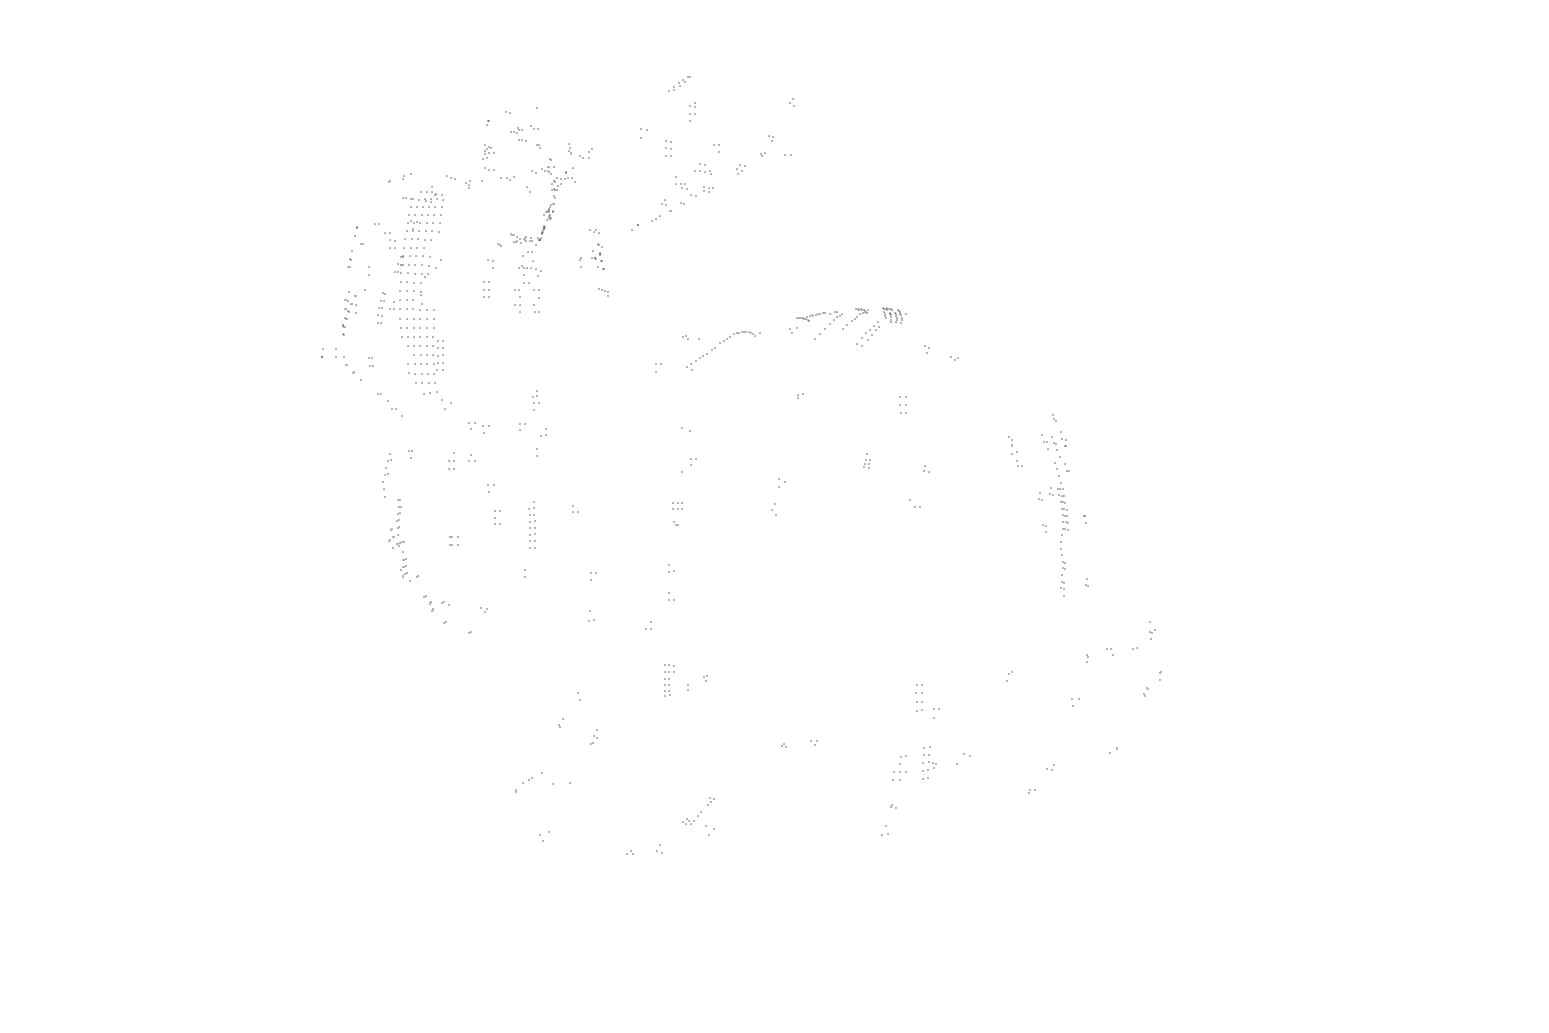
\includegraphics[width = .48\linewidth]{images/incrementalLoading/95}%
	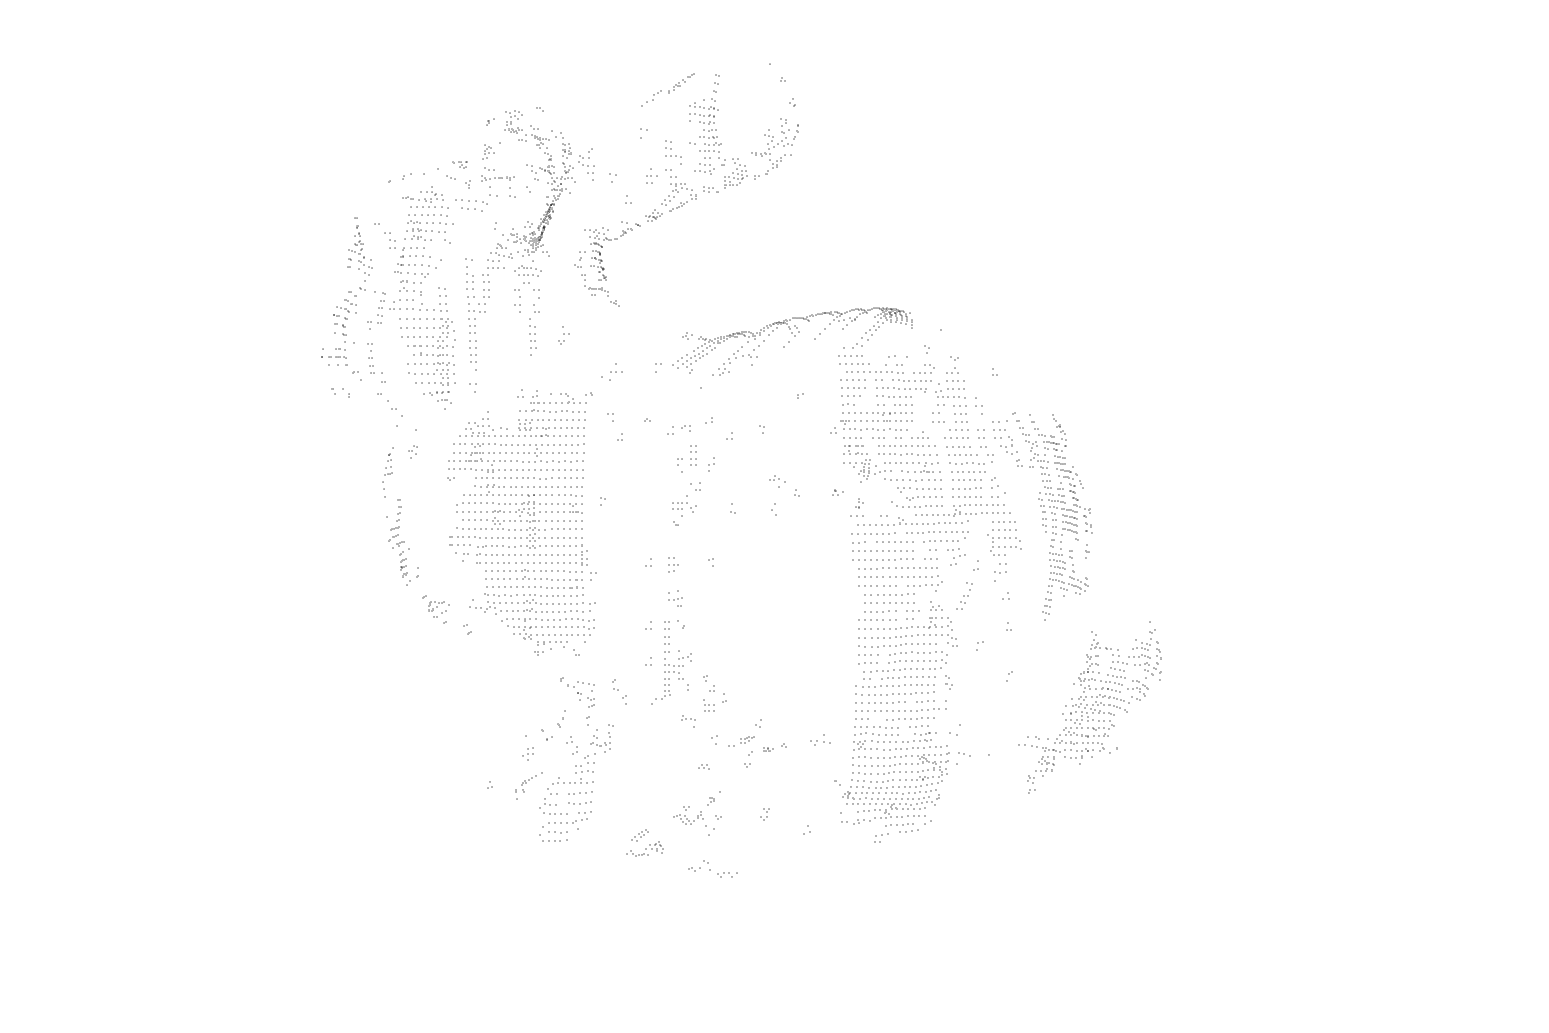
\includegraphics[width = .48\linewidth]{images/incrementalLoading/97}
	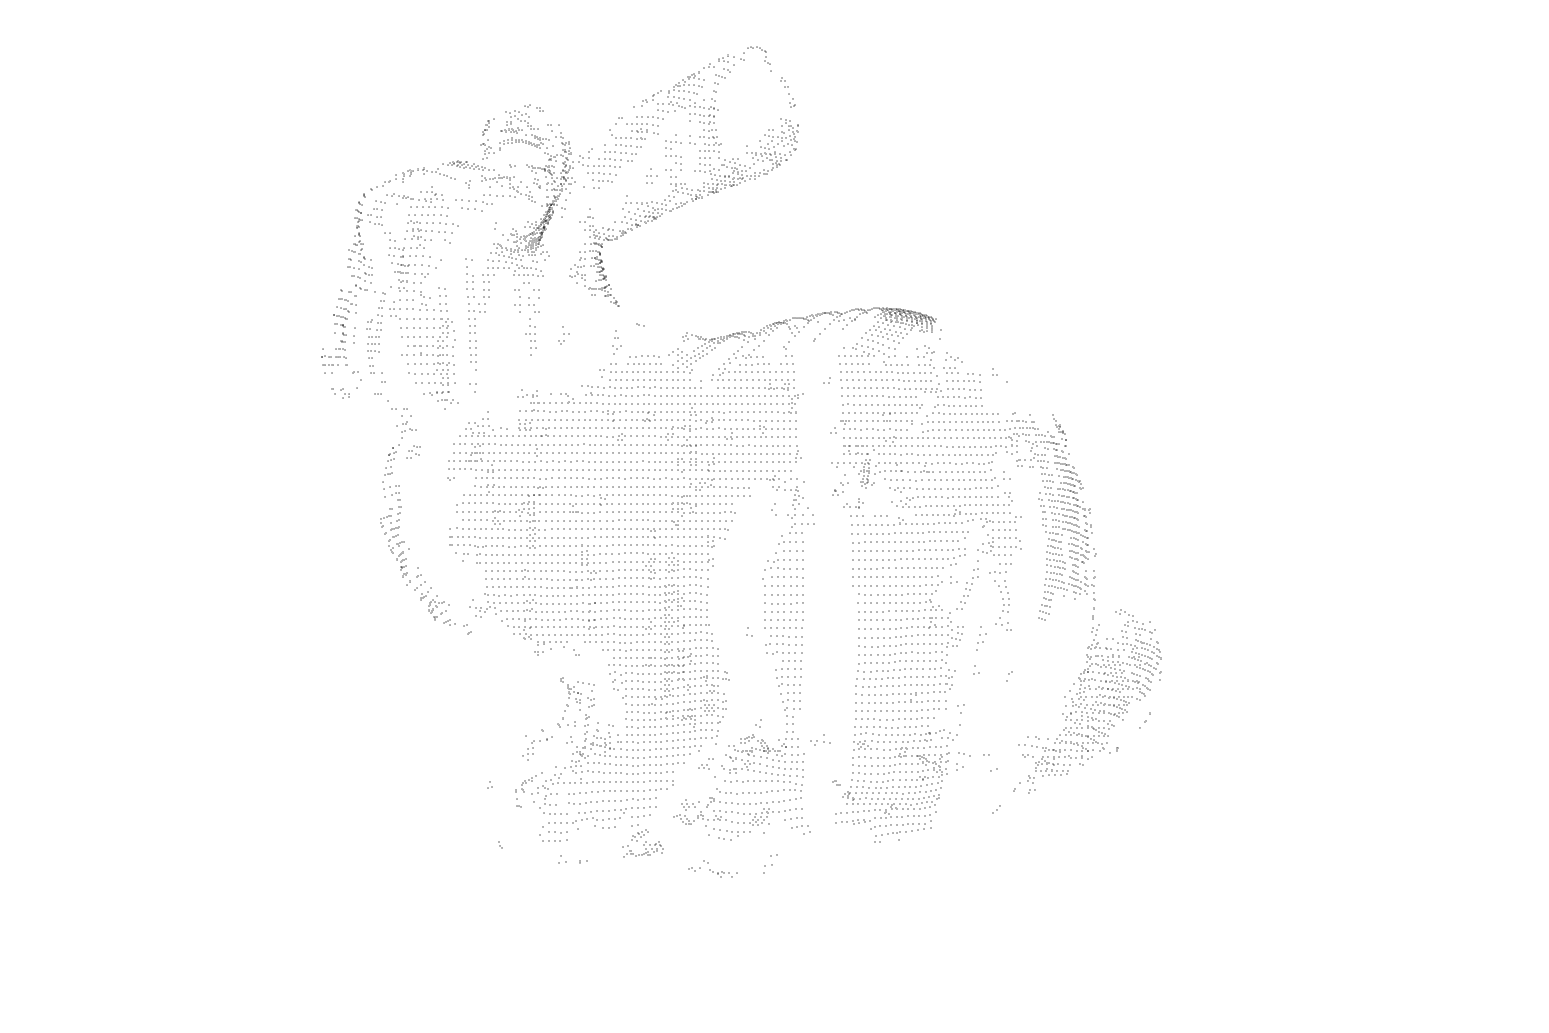
\includegraphics[width = .48\linewidth]{images/incrementalLoading/99}%
	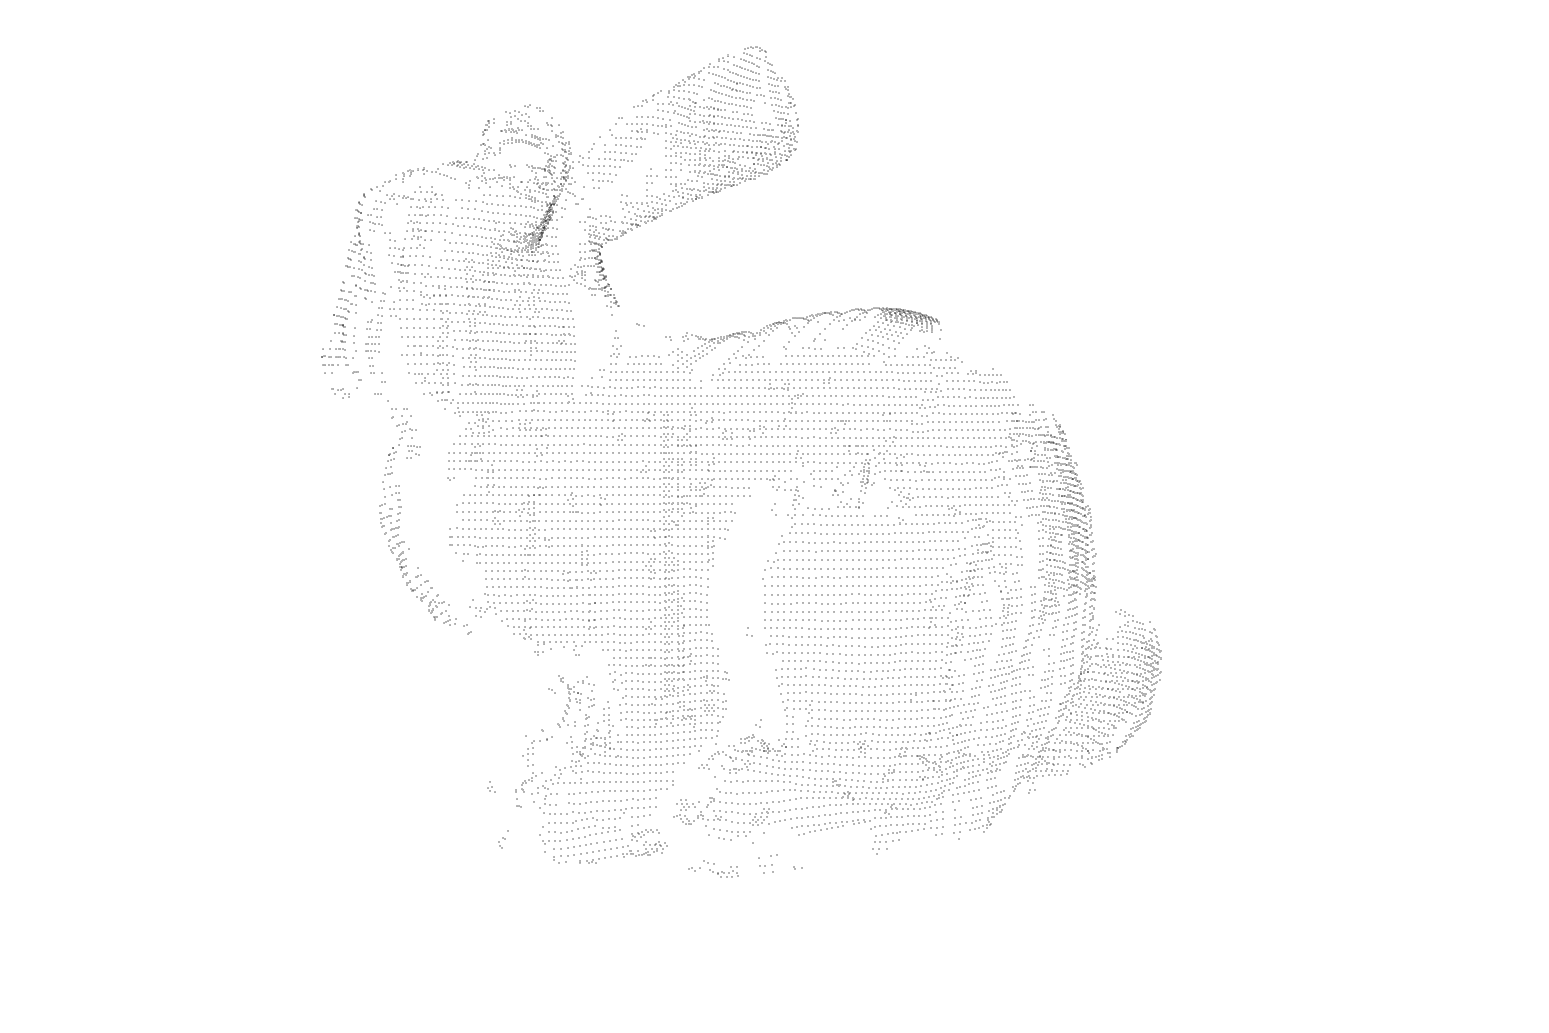
\includegraphics[width = .48\linewidth]{images/incrementalLoading/101}
	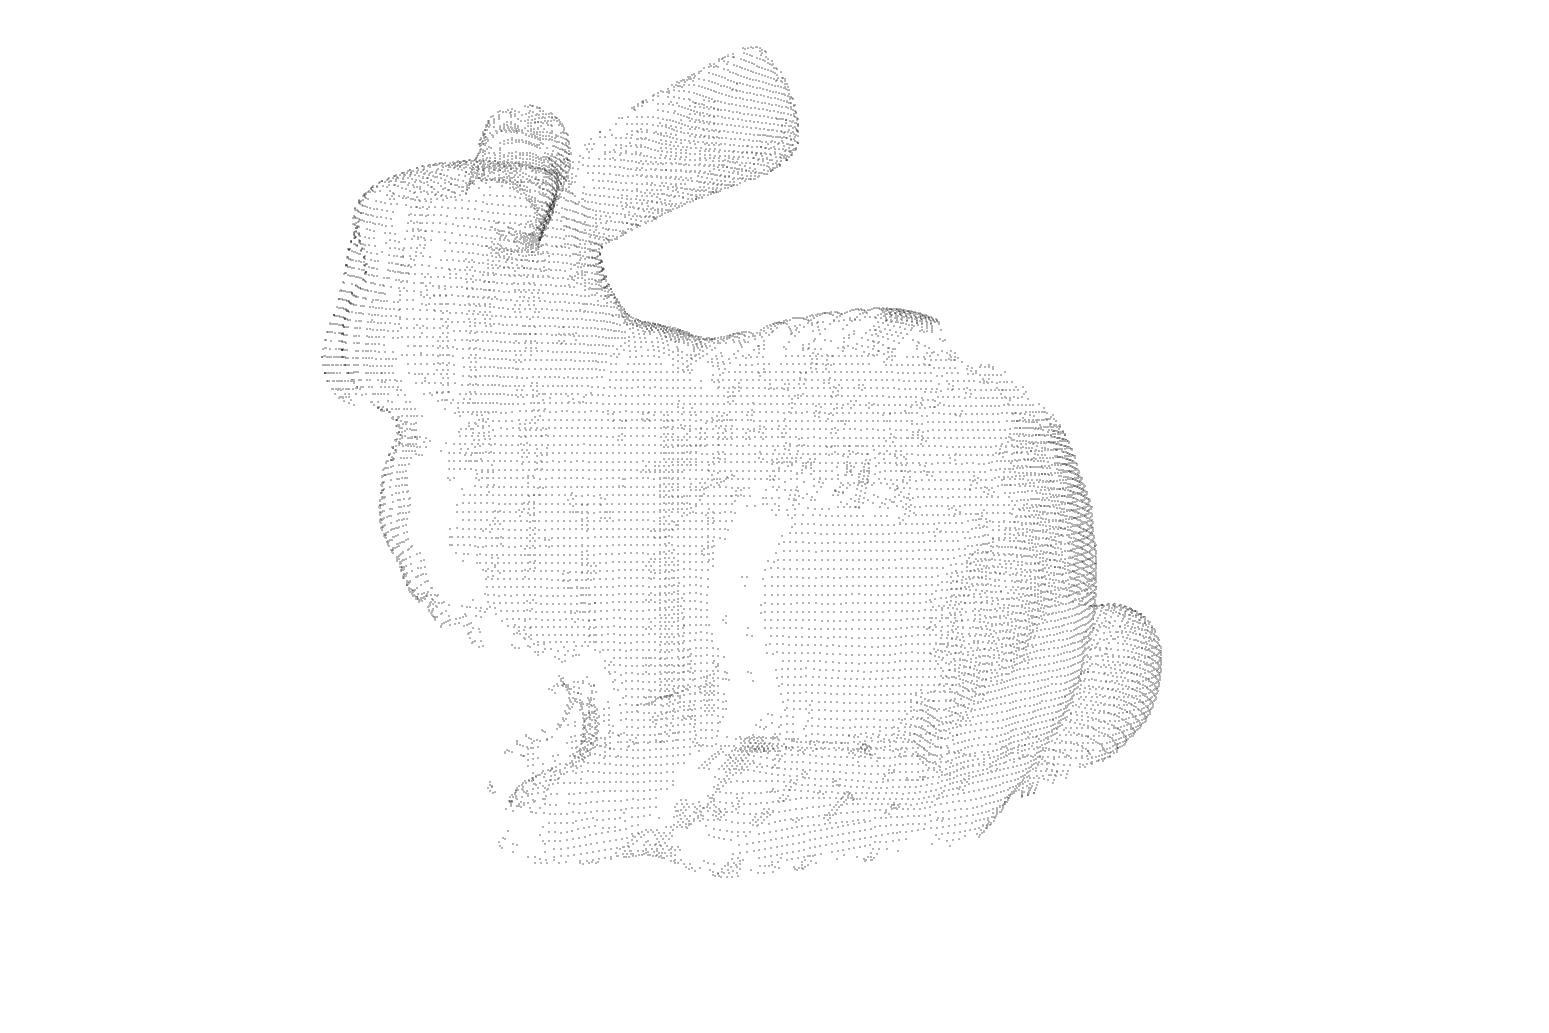
\includegraphics[width = .48\linewidth]{images/incrementalLoading/105}%
	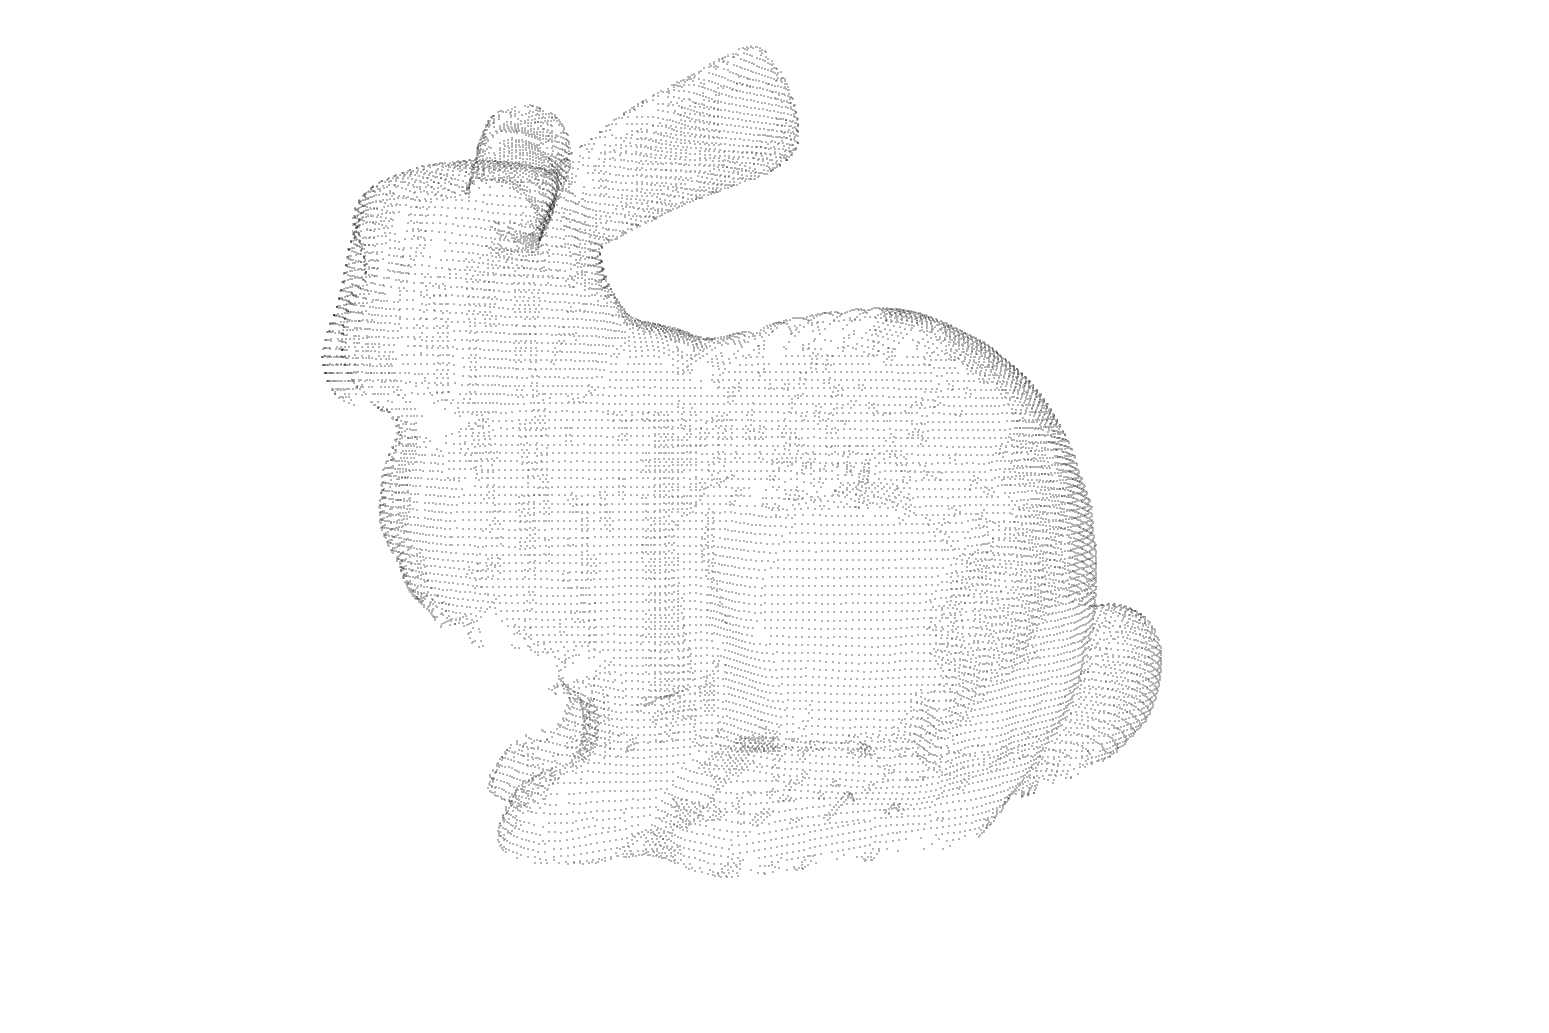
\includegraphics[width = .48\linewidth]{images/incrementalLoading/107}
	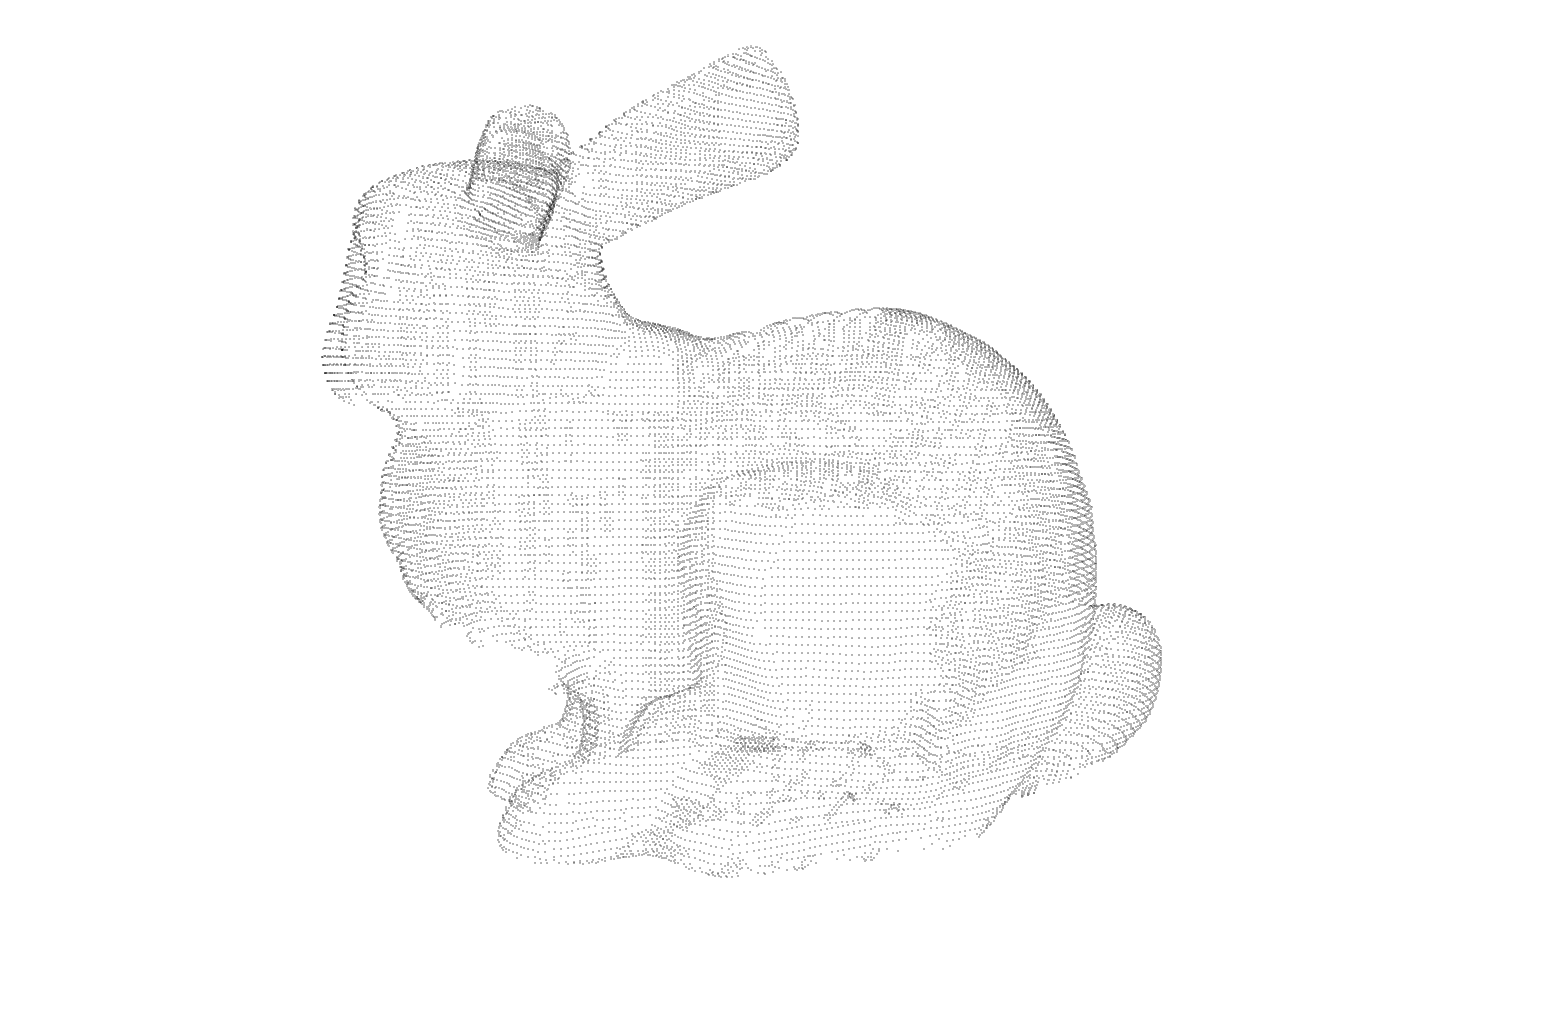
\includegraphics[width = .48\linewidth]{images/incrementalLoading/109}%
	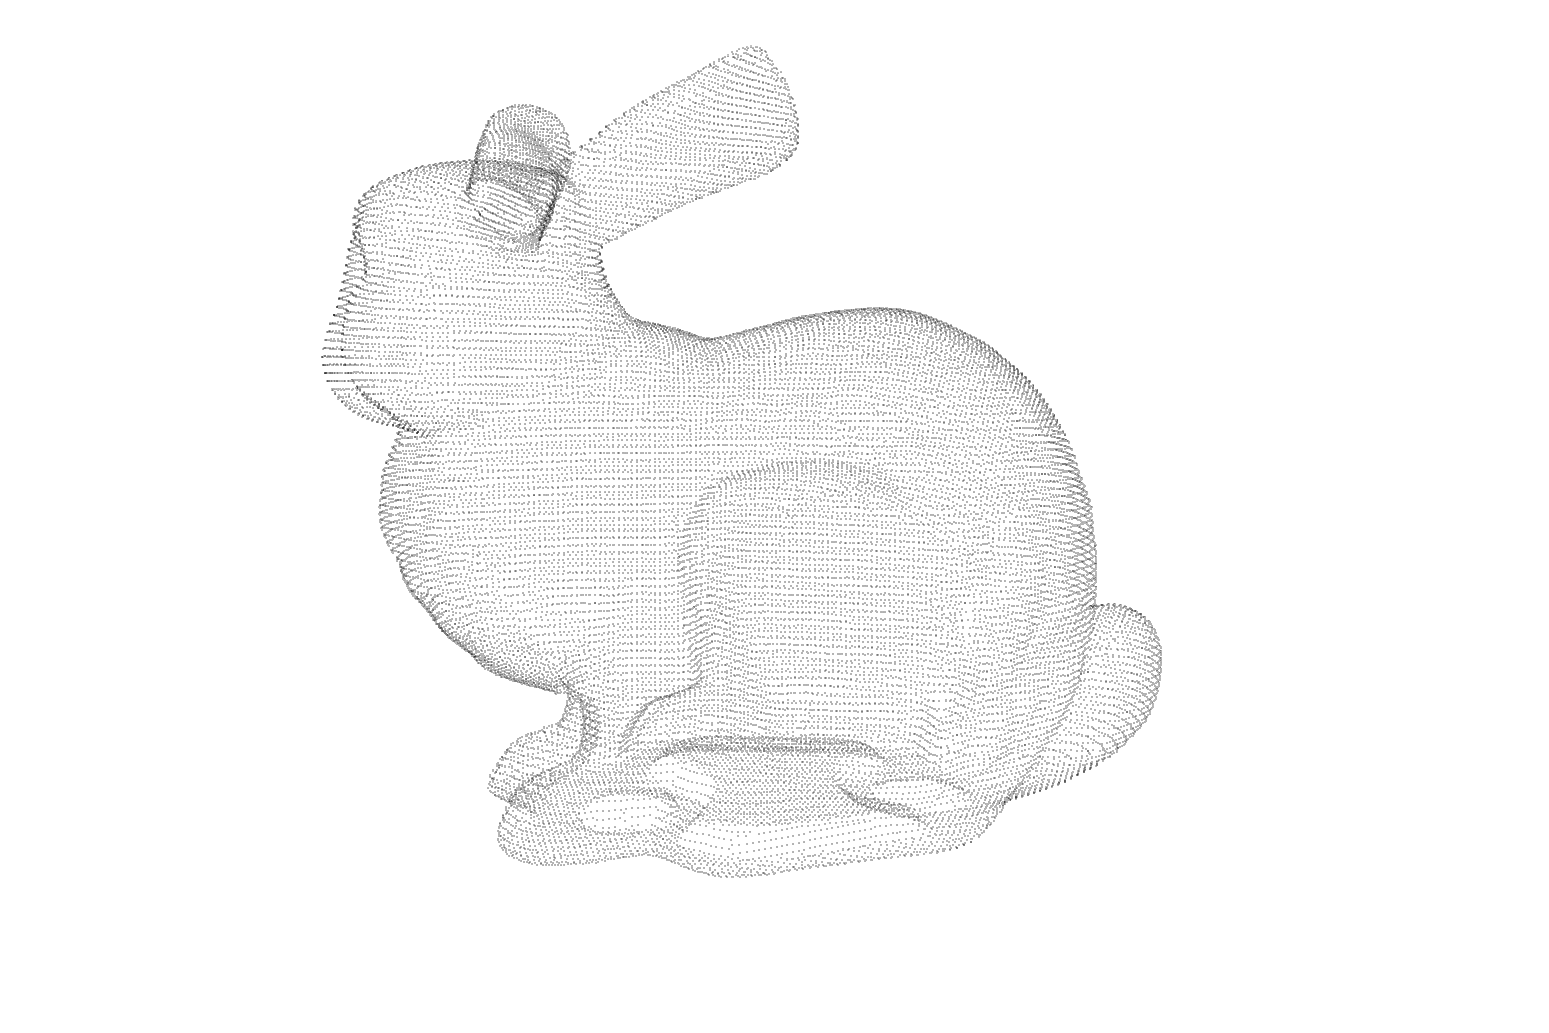
\includegraphics[width = .48\linewidth]{images/incrementalLoading/115}
	\caption{Inkrementelles Nachladen von Punkten der Wolke in das LDI.}%
	\label{img:incload}
\end{figure}

Das Ziel der Entkopplung zwischen Datenverarbeitung und Anzeige wurde
größtenteils erreicht. So ist mit einem optimierten Kompilat der Implementation
keine messbare Verzögerung zwischen dem erzeugen Punktwolkenanfrage und seiner
Fertigstellung wahrzunehmen. Ein Debugbuild zeigt auf anschauliche Weise, wie
das Einfügen von Punkten aus der Wolke abläuft (siehe
Abbildung~\ref{img:incload}). So ist erkennbar, dass zunächst kleine
Punktgruppen quasi zufällig geladen werden. Wenig später sind nahezu
rechteckige Patches auf der Oberfläche erkennbar. Daraufhin ist eine
Objektoberfläche bereits wahrnehmbar. Es ist jedoch auffällig, dass bis zuletzt
einzelne Reihen von Punkten unaufgefüllt bleiben.

Diese Effekte lassen sich durch zwei primäre Ursachen erklären. So wird durch
Speicherung der Punktwolke als Datei eine Serialisierung durchgeführt. Unter
der Annahme, dass die \texttt{point\_cloud} diese Anordnung auch intern
verwendet, unterliegen die Punkte der Wolke dadurch einer impliziten
Reihenfolge. Da an allen Übergabepunkten der Implementation die Verarbeitung
seriell erfolgt, bleibt diese Reihenfolge somit in einem lokalen Intervall
erhalten. Es ist außerdem möglich, dass beim ursprünglichen Speichern eine
gewisse Anordnung erreicht werden sollte. So ist es denkbar, dass verschiedene
Qualitätsstufen nacheinander gespeichert wurden. Bei Bildern die über langsame
Netzwerke übertragen werden, wird häufig Interlacing\footnote{Das
PNG-Bildformat bietet zum Beispiel ein Interlacing nach Adam7 an.} eingesetzt
um eine initale Approximation des Inhalts möglichst frühzeitig anzeigen zu
können. Da das verwendete Modell des Stanford Bunny 1993 (siehe~\cite{bunny})
angefertigt wurde, ist ein ähnliches Verfahren wahrscheinlich.

Des Weiteren sind die Verarbeitungsschritte durch die
\texttt{std::timed\_mutex} zeitlich aneinander gekoppelt. So hat die Framerate
einen direkten Einfluss auf die Größe der Anfragen und die Menge an Punkten,
die auf einmal in das LDI kopiert werden können. Es ist denkbar dass hierbei
Oszillationseffekte durch die sog. Lock Contention auftreten. So ist ein Mutex
eine Betriebssystemressource und muss durch eben dieses verwaltet werden. Wie
jedoch bekannt ist, sind alle Aufrufe, die in den Kernel Adressraum führen,
äußerst teuer. Daraus folgen in Überlastungssituationen überproportional
ansteigende Laufzeitkosten während der Reservierung des Mutex. Dies hat die
Wechselwirkung zur Folge, dass während einer Überlastung die Zeit für
Anfragenerstellung und Ausführung sich verringert. Diese Situation wird jedoch
durch den Prozess-Scheduler des Betriebssystems schubweise entschärft. Dadurch
sind wieder längere Zeitabschnitte zur Abarbeitung möglich. Lange gehaltene
exklusive Abschnitte führen jedoch wieder zu der oben begonnenen Überlastung.
Diese Beobachtung bestätigt sich auch durch einen sägezahnartigen
Auslastungsverlauf der CPU.\@ Als direkte Folge dieser schwankenden
Zeitintervalle sind auch die zusammenhängenden Bereiche der Wolke einer
zyklischen Schwankung ausgesetzt.

Trotz Entkopplung des Nachladens und der Anzeige versagt die Implementation bei
größeren Datenwolken wie dem Lego 3D Scans (rund 52 MB). So entstehen initiale
Verzögerungen und es dauert ca. 8 Sekunden bis alle sichtbaren Punkte angezeigt
werden (Haswell i7 4790K, 16 GB DDR3, Maxwell GTX 980). Es kann zwar eine
nahezu konstante Bildrate gehalten werden, die qualitativen Einbußen sind
jedoch gravierend (siehe Abbildung~\ref{img:lego}). Auf mögliche Gründe wird im
Abschnitt~\ref{sec:discussion} eingegangen.

\begin{figure}
	\centering
	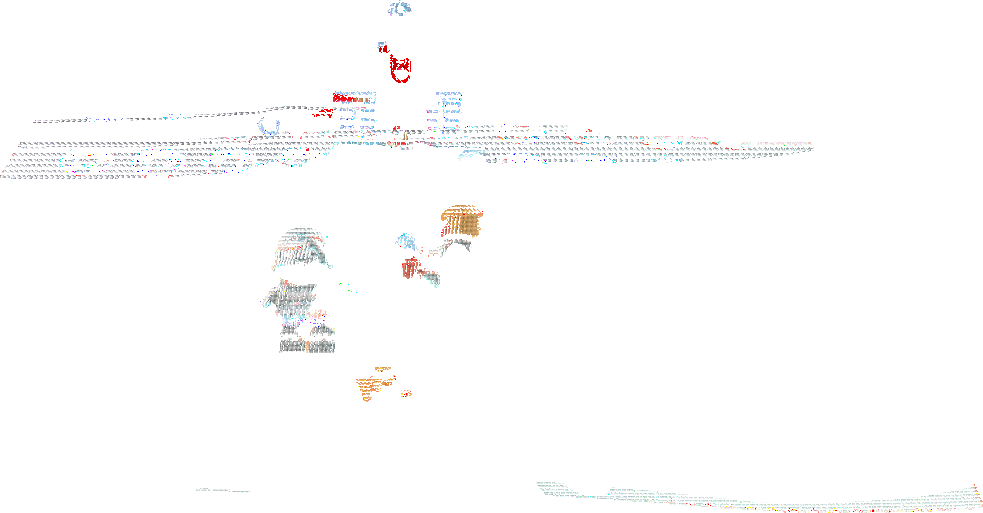
\includegraphics[width = \linewidth]{images/Lego/126}
	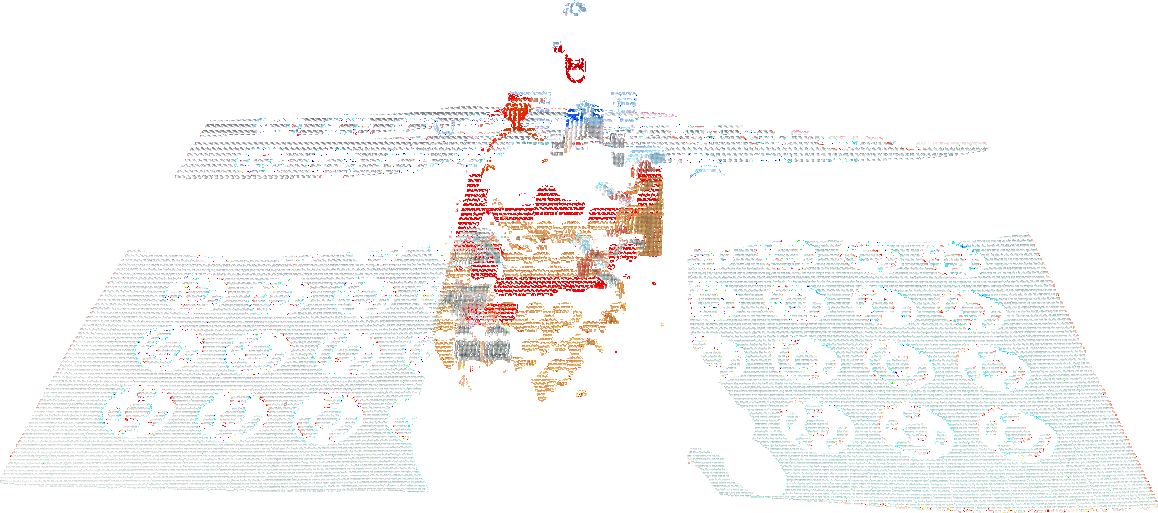
\includegraphics[width = \linewidth]{images/Lego/150}
	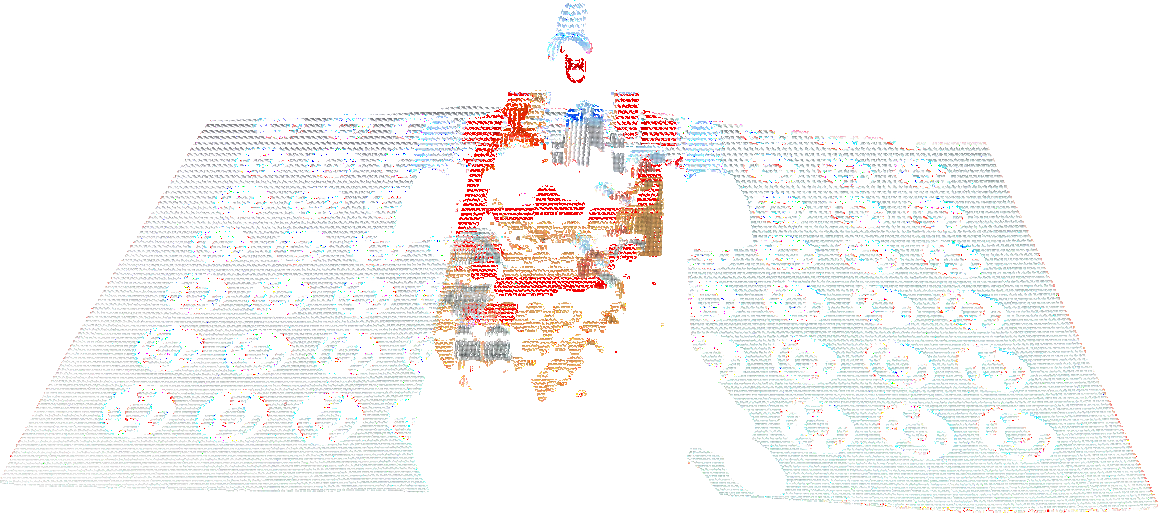
\includegraphics[width = \linewidth]{images/Lego/170}
	\caption{Inkrementelles Rendern des Lego 3D Scans.
	Das schichtweise Nachladen erfolgt über einen Zeitraum von ca. 8 Sekunden.}%
	\label{img:lego}
\end{figure}

\section{Qualitative Betrachtung}

Da die in der Implementation verwendete Form des LDI weiterhin Punkte und nicht
reine Bildpixel verwaltet, führt dies zur Überlegung den vorhandenen
Punktrenderer des CGV Frameworks wiederzuverwenden. Deshalb ist ein direkter
Vergleich zweier fertig gestellter Bilder nicht aufschlussreich, da sie
letztendlich durch den gleichen Vorgang gezeichnet wurden. Da das
Punktrendering außerdem nur einzelne Pixel einfärbt, sind klassische
Vergleichsmetriken, wie das Differenzbild ohne Anpassung nicht sinnvoll. Ein
Unterschied zwischen beiden Renderingverfahren würde sich nur durch
Abweichungen in den Bildpositionen bemerkbar machen. Deshalb wird vor dem
eigentlichen Vergleich ein Gaußfilter mit einem Durchmesser von 5 Pixeln auf
beide Bilder angewandt. Somit wird eine punktuelle Diskrepanz über einen
lokalen Bereich gestreut.

\begin{figure}
	\centering
	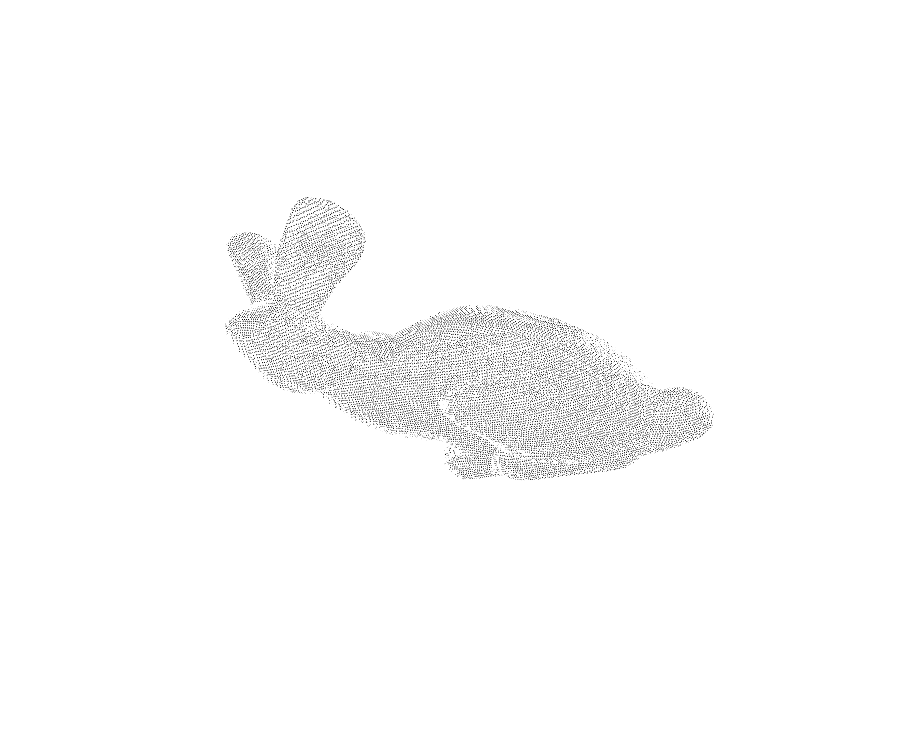
\includegraphics[width = .48\linewidth]{images/distortion/239}%
	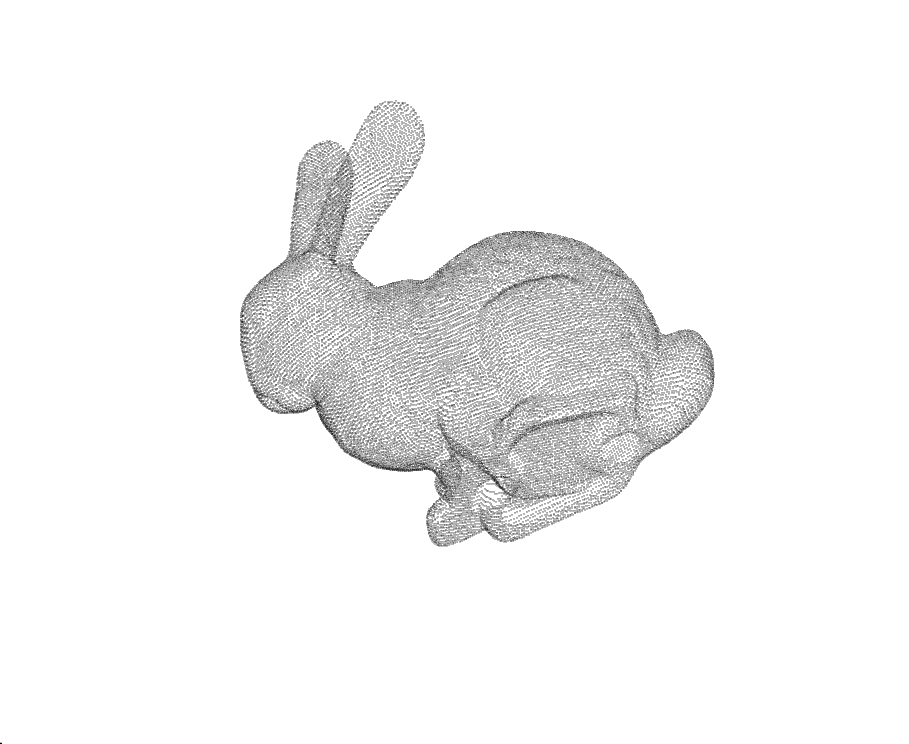
\includegraphics[width = .48\linewidth]{images/distortion/241}
	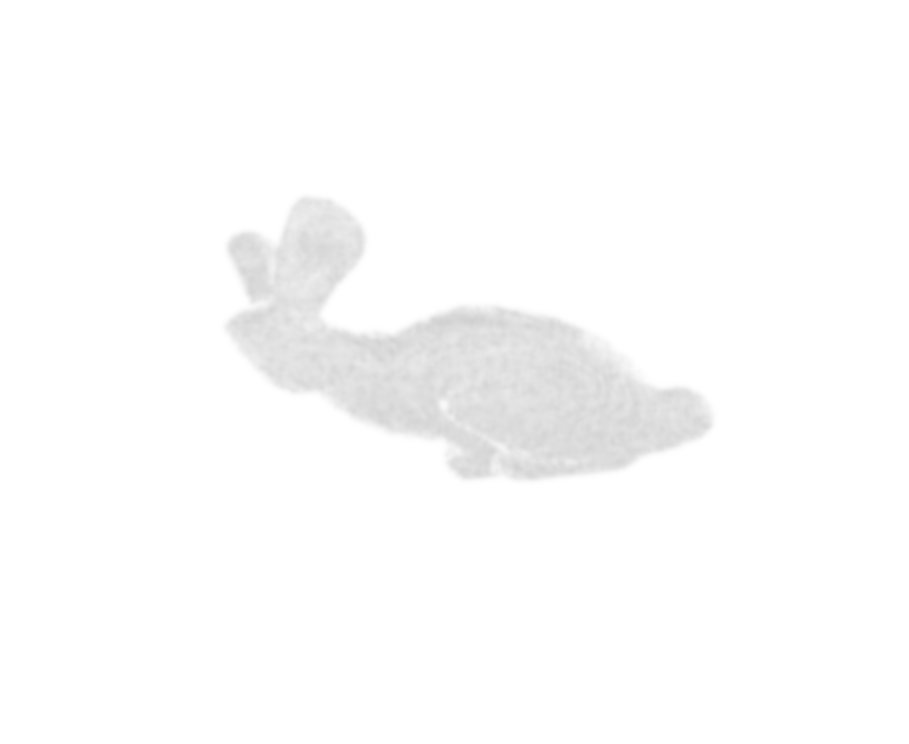
\includegraphics[width = .48\linewidth]{images/distortion/239_filtered}%
	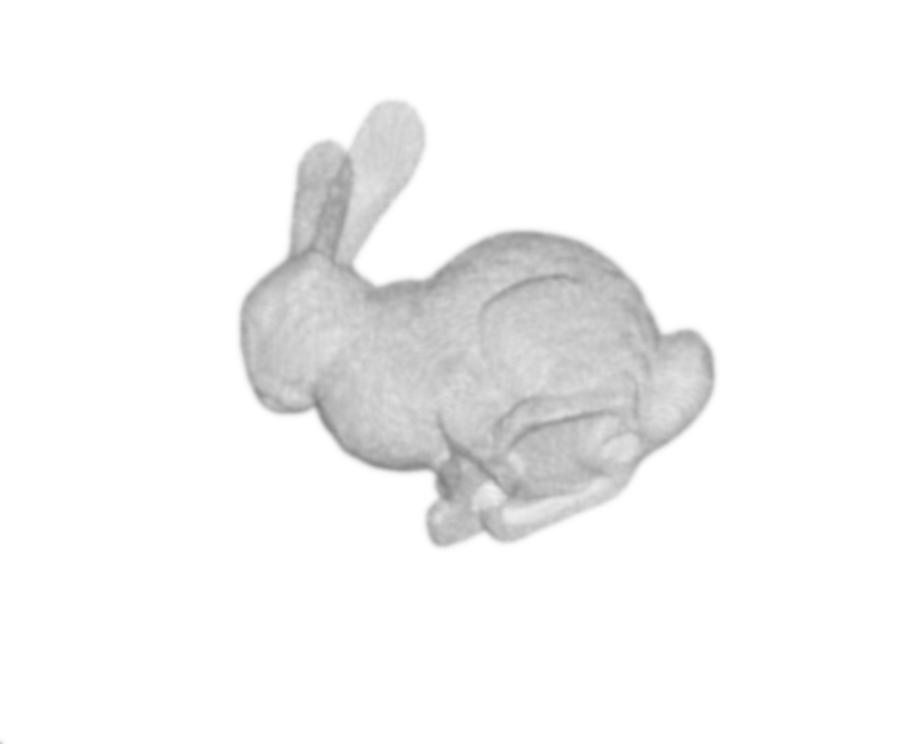
\includegraphics[width = .48\linewidth]{images/distortion/241_filtered}
	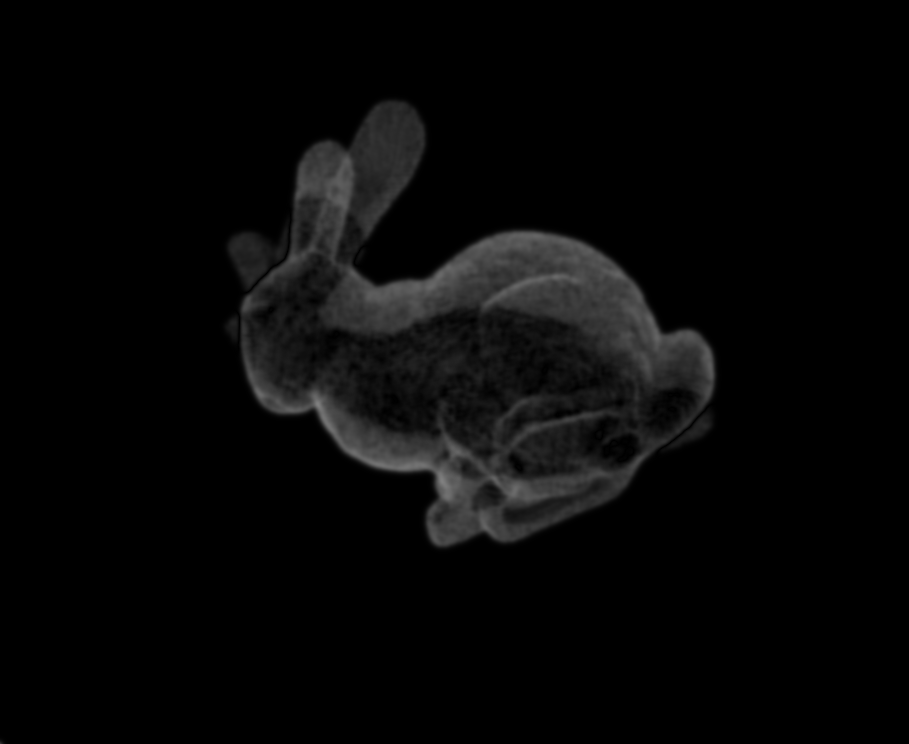
\includegraphics[width = .48\linewidth]{images/distortion/diff}
	\caption{Verzerrungsartefakte bei starken Unterschieden in der Sichtposition.
	Die linke Seite entstand aus dem Morphing, die Rechte aus einem neu 
	generierten LDI aus dieser Kameraperspektive. Das untere Differenzbild zeigt
	den Unterschied beider Ansichten auf. Schwarze Bereiche weisen identische 
	Luminanz auf, weiße Bereich markieren eine Luminanzabweichung.}%
	\label{img:distortion}
\end{figure}

Ein gravierender Qualitätsverlust entsteht beim wiederholten Morphen von
Ansichten mit sich stark unterscheidenden Positionen und Winkeln.
Abbildung~\ref{img:distortion} stellt einen solchen Extremfall dar. Das
Differenzbild zeigt deutliche Abweichungen in der Silhouette des Modells.
Außerdem interessant ist der Unterschied in der Punktdichte der beiden Bilder.
So sind in der Differenz graue Bereiche mit unterschiedlicher Helligkeit und
somit variierender Diskrepanz sichtbar. Daraus folgt, dass durch das LDI
Morphing die effektive Punktdichte komprimiert wird. Dies ist eventuell durch
unvorteilhafte Rundung von Bildpositionen erklärbar. So wird während des
Morphings mit 32 Bit Gleitkommazahlen gearbeitet. In Abhängig der
Rundungseinstellungen der CPU kann diese in einem simplen Abschneiden der
Nachkommastellen resultieren. Eine konventionelle Rundung durch die Intervalle
\( \left(0, 0.5\right) \) und \( \left[0.5, 1\right] \) würde den
durchschnittlichen quadrierten Abstand zwischen eigentlicher und endgültiger
Position verringern.

Um solche Situationen zu provozieren, werden wiederholt
ruckartige Mausbewegungen ausgeführt um eine möglichst große Abweichung
zwischen zwei Bildern zu erreichen. Die dargestellte Verzerrung tritt immer
dann auf, wenn unvollständig gemorphte LDIs bereits zur Generation neuer
Ansichten genutzt werden. Auch wenn diese Effekte bei normaler Nutzung im CGV
Viewer nicht auftreten, so stellen sie doch einen gravierenden Mangel dar. Bei
der angedachten Nutzung durch ein HMD ist die Wahrscheinlichkeit von
ruckartigen Kopfbewegungen deutlich höher. Das Auftreten in eben diesem Moment
ist jedoch fatal, da dem Gehirn somit kurzeitig inkonsistente visuelle
Informationen geliefert werden. Dies kann im schlimmsten Fall zu
Gleichgewichtsstörungen führen.

\section{Diskussion}%
\label{sec:discussion}

Zunächst ist festzustellen, dass das erwünschte Ziel von 90 Bildern pro Sekunde
nicht erreicht wurde. Obwohl Datenverarbeitung und Rendering nebenläufig
ausgeführt werden, reicht das Zeitbudget von ca. \SI{11,1}{\milli\second} nicht
aus, um alle Punkte zu zeichnen. Die initiale Annahme, dass der Rechenaufwand
des Morphings den Flaschenhals darstellt, hat sich nicht bewahrheitet. So
wurden testweise Teile der Berechnung mit intrinsischen SSE Funktionen des
Compilers ausgetauscht. Diese führten jedoch zu keinem messbaren Vorteil.
Daraufhin wurde die Implementation mehrfach mit einem Laufzeit-Profiler
untersucht. Dadurch konnten überflüssige Aufrufe entfernt werden und die
Ausdehnung von kritischen Bereichen verkleinert werden. Diese Maßnahmen
reichten jedoch nicht aus, um dass FPS Ziel zu erreichen. Die hauptsächlichen
Verbraucher von Aufrufzeit sind Speicherzugriffe und zu einem geringeren Teil
Kernelfunktionen. Dies führt zu der Festellung, das die Implementation des LDIs
und der Morphinggleichung auf der CPU fehlplatziert sind. So erreicht
DDR3--1600 Hauptspeicher nur einen Durchsatz von 12,8 GB/s. Auf Grafikkarten
wird jedoch GDDR5 o.Ä.\ benutzt und erreicht Größenordnungen von 224,4 GB/s
(GTX 980). Mit diesem Umstand erscheint eine Speicherung des LDIs direkt auf
der GPU und ein Morphing durch dedizierte Shader erfolgsversprechender. Die
Implementation auf der CPU entstand jedoch aus der Motivation, die erweiterten
Fähigkeiten des bestehenden CGV Renderers wiederzuverwenden.

Es hat sich auch als Nachteilig erwiesen, dass die benutzte Klasse zum Laden
der Punktwolke die gesamte Datei in den Speicher lädt. Dies führt bei
ausreichend großen Punktwolken zu einem Abbruch des Programms wegen
Speichermangel. Dieser Umstand lässt sich durch eine In-Memory Kompression mit
z.B. LZ4 abschwächen. Eine endgültige Lösung stellt jedoch nur die Nutzung
einer Verwaltungsstruktur für quasi wahlfreien Zugriff auf eine Punktwolke im
Dateisystem dar.

Eine weitere Modifikation der vorgestellten Implementation kann mit dem
kommenden C++20 Standard umgesetzt werden. Dieser führt sog. Coroutines in den
Sprachkern ein und ermöglicht dadurch eine Nebenläufigkeit, die nicht auf
Betriebssystemressourcen angewiesen ist. Indem der Aufrufzustand einer Funktion
unabhängig von Aufrufstack gespeichert wird, können Funktionen beliebig oft
unterbrochen und wieder aufgenommen werden. Dadurch wird eine Programmstruktur
möglich, welche von den Kostenüberlegungen des Mutex Gebrauchs befreit sind. So
wäre es zum Beispiel denkbar, dass der Renderingprozess direkt mit der
Granularität von einem Punkt die Datenanfragen konsumiert. Da keine
Mutexvariablen genutzt werden müssen, wäre der Zeitaufwand vernachlässigbar und
die beiden Prozesse würden quasi parallel ablaufen. Diese Modifikation ist
außerdem unabhängig von der vorgeschlagenen Umsetzung auf der GPU und kann
diese sogar weiter verbessern.

\chapter{Fazit}

Die vorliegende Arbeit hat die Layered Depth Images als neuartigen
Renderingansatz für Punktwolken untersucht. Dafür wurde eine CPU gestützte
Implementation angefertigt und ausgewertet. Auch wenn das geforderte Framerate
Ziel nicht erreicht wurde, gibt die Implementation einen Ausblick auf die
Vorteile von LDI basierten Renderingverfahren.

Wie bereits aufgezeigt, erscheint die GPU basierte LDI Implementation als
zukünftige Untersuchung äußerst lohnenswert. Die vorgestellte CPU Lösung kann
zwar durch die Wiederverwendung des bestehenden Punktrenderer einfach umgesetzt
werden, scheitert jedoch an den enormen Speicherdurchsatz-Forderungen, die mit
jedem gerenderten Bild erneut auftreten. Zukünftige Umsetzungen sollten daher
ein besonderes Augenmerk auf die effiziente Kommunikation zwischen CPU und GPU
legen. Eine Vorhaltung des LDI im Grafikspeicher scheint unabdingbar und eine
fortgeschrittene Art des Datenaustausches angebracht. Dafür bieten sich zum
Beispiel sog. Persistent Mapped Buffer Objects an. In Abhängigkeit der OpenGL
Implementation lassen sich diese Puffer sehr effizient austauschen oder
aktualisieren.

Ein möglicher Ansatz zur Weiterenwicklung von LDIs lässt sich mit dem
generellen Erfolg von HMDs erkennen. Da für diese Anwendung stereoskopische
Bilder generiert werden müssen, entsteht die Frage ob LDIs auf diesen
Spezialfall optimiert werden können. So müssten mit der aktuellen
Implementation entweder beide Stereobilder aus dem Mittelpunkt zwischen beiden
Augen gemorpht werden oder zwei separate LDIs gespeichert werden. Eventuell
ließe sich anstatt der Tiefe die generalisierte Disparität für jeden Punkt
speichern und die Morphing Gleichung entsprechend anpassen. Dies würde eine
elegantere Lösung des Stereofalls ermöglichen.

\end{document}
